\documentclass[twoside]{book}

% Packages required by doxygen
\usepackage{calc}
\usepackage{doxygen}
\usepackage{graphicx}
\usepackage[utf8]{inputenc}
\usepackage{makeidx}
\usepackage{multicol}
\usepackage{multirow}
\usepackage{textcomp}
\usepackage[table]{xcolor}

% Font selection
\usepackage[T1]{fontenc}
\usepackage{mathptmx}
\usepackage[scaled=.90]{helvet}
\usepackage{courier}
\usepackage{amssymb}
\usepackage{sectsty}
\renewcommand{\familydefault}{\sfdefault}
\allsectionsfont{%
  \fontseries{bc}\selectfont%
  \color{darkgray}%
}
\renewcommand{\DoxyLabelFont}{%
  \fontseries{bc}\selectfont%
  \color{darkgray}%
}

% Page & text layout
\usepackage{geometry}
\geometry{%
  a4paper,%
  top=2.5cm,%
  bottom=2.5cm,%
  left=2.5cm,%
  right=2.5cm%
}
\tolerance=750
\hfuzz=15pt
\hbadness=750
\setlength{\emergencystretch}{15pt}
\setlength{\parindent}{0cm}
\setlength{\parskip}{0.2cm}
\makeatletter
\renewcommand{\paragraph}{%
  \@startsection{paragraph}{4}{0ex}{-1.0ex}{1.0ex}{%
    \normalfont\normalsize\bfseries\SS@parafont%
  }%
}
\renewcommand{\subparagraph}{%
  \@startsection{subparagraph}{5}{0ex}{-1.0ex}{1.0ex}{%
    \normalfont\normalsize\bfseries\SS@subparafont%
  }%
}
\makeatother

% Headers & footers
\usepackage{fancyhdr}
\pagestyle{fancyplain}
\fancyhead[LE]{\fancyplain{}{\bfseries\thepage}}
\fancyhead[CE]{\fancyplain{}{}}
\fancyhead[RE]{\fancyplain{}{\bfseries\leftmark}}
\fancyhead[LO]{\fancyplain{}{\bfseries\rightmark}}
\fancyhead[CO]{\fancyplain{}{}}
\fancyhead[RO]{\fancyplain{}{\bfseries\thepage}}
\fancyfoot[LE]{\fancyplain{}{}}
\fancyfoot[CE]{\fancyplain{}{}}
\fancyfoot[RE]{\fancyplain{}{\bfseries\scriptsize Generated on Sun Oct 11 2015 22\-:33\-:17 for G\-N\-U Octave by Doxygen }}
\fancyfoot[LO]{\fancyplain{}{\bfseries\scriptsize Generated on Sun Oct 11 2015 22\-:33\-:17 for G\-N\-U Octave by Doxygen }}
\fancyfoot[CO]{\fancyplain{}{}}
\fancyfoot[RO]{\fancyplain{}{}}
\renewcommand{\footrulewidth}{0.4pt}
\renewcommand{\chaptermark}[1]{%
  \markboth{#1}{}%
}
\renewcommand{\sectionmark}[1]{%
  \markright{\thesection\ #1}%
}

% Indices & bibliography
\usepackage{natbib}
\usepackage[titles]{tocloft}
\setcounter{tocdepth}{3}
\setcounter{secnumdepth}{5}
\makeindex

% Custom commands
\newcommand{\clearemptydoublepage}{%
  \newpage{\pagestyle{empty}\cleardoublepage}%
}


%===== C O N T E N T S =====

\begin{document}

% Titlepage & ToC
\pagenumbering{roman}
\begin{titlepage}
\vspace*{7cm}
\begin{center}%
{\Large G\-N\-U Octave \\[1ex]\large 4.\-0 }\\
\vspace*{1cm}
{\large Generated by Doxygen 1.8.6}\\
\vspace*{0.5cm}
{\small Sun Oct 11 2015 22:33:17}\\
\end{center}
\end{titlepage}
\clearemptydoublepage
\tableofcontents
\clearemptydoublepage
\pagenumbering{arabic}

%--- Begin generated contents ---
\chapter{Octave with Doxygen}
\label{index}Here I generate Octave documentation with the Doxygen. Ealier I does not know about doxygen how to use it, so I start from doxygen with python . I generate documentation for python files and I face minor problems But solve them very quicky. But my work is to generate documentation for octave files, Hence I generate it. 
\chapter{Hierarchical Index}
\section{Class Hierarchy}
This inheritance list is sorted roughly, but not completely, alphabetically\-:\begin{DoxyCompactList}
\item \contentsline{section}{top}{\pageref{classtop}}{}
\begin{DoxyCompactList}
\item \contentsline{section}{middle}{\pageref{classmiddle}}{}
\begin{DoxyCompactList}
\item \contentsline{section}{bottom}{\pageref{classbottom}}{}
\end{DoxyCompactList}
\end{DoxyCompactList}
\end{DoxyCompactList}

\chapter{Class Index}
\section{Class List}
Here are the classes, structs, unions and interfaces with brief descriptions\-:\begin{DoxyCompactList}
\item\contentsline{section}{\hyperlink{classpython__class_1_1student}{python\-\_\-class.\-student} }{\pageref{classpython__class_1_1student}}{}
\end{DoxyCompactList}

\chapter{File Index}
\section{File List}
Here is a list of all files with brief descriptions\-:\begin{DoxyCompactList}
\item\contentsline{section}{\hyperlink{calculator_8py}{calculator.\-py} }{\pageref{calculator_8py}}{}
\item\contentsline{section}{\hyperlink{class__concept_8py}{class\-\_\-concept.\-py} }{\pageref{class__concept_8py}}{}
\item\contentsline{section}{\hyperlink{demodatabase_8py}{demodatabase.\-py} }{\pageref{demodatabase_8py}}{}
\item\contentsline{section}{\hyperlink{file_8py}{file.\-py} }{\pageref{file_8py}}{}
\item\contentsline{section}{\hyperlink{hello_8py}{hello.\-py} }{\pageref{hello_8py}}{}
\item\contentsline{section}{\hyperlink{if__demo_8py}{if\-\_\-demo.\-py} }{\pageref{if__demo_8py}}{}
\item\contentsline{section}{\hyperlink{pdemo_8py}{pdemo.\-py} }{\pageref{pdemo_8py}}{}
\item\contentsline{section}{\hyperlink{python__class_8py}{python\-\_\-class.\-py} }{\pageref{python__class_8py}}{}
\end{DoxyCompactList}

\chapter{Class Documentation}
\section{bottom Class Reference}
\label{classbottom}\index{bottom@{bottom}}


Inheritance diagram for bottom\-:\nopagebreak
\begin{figure}[H]
\begin{center}
\leavevmode
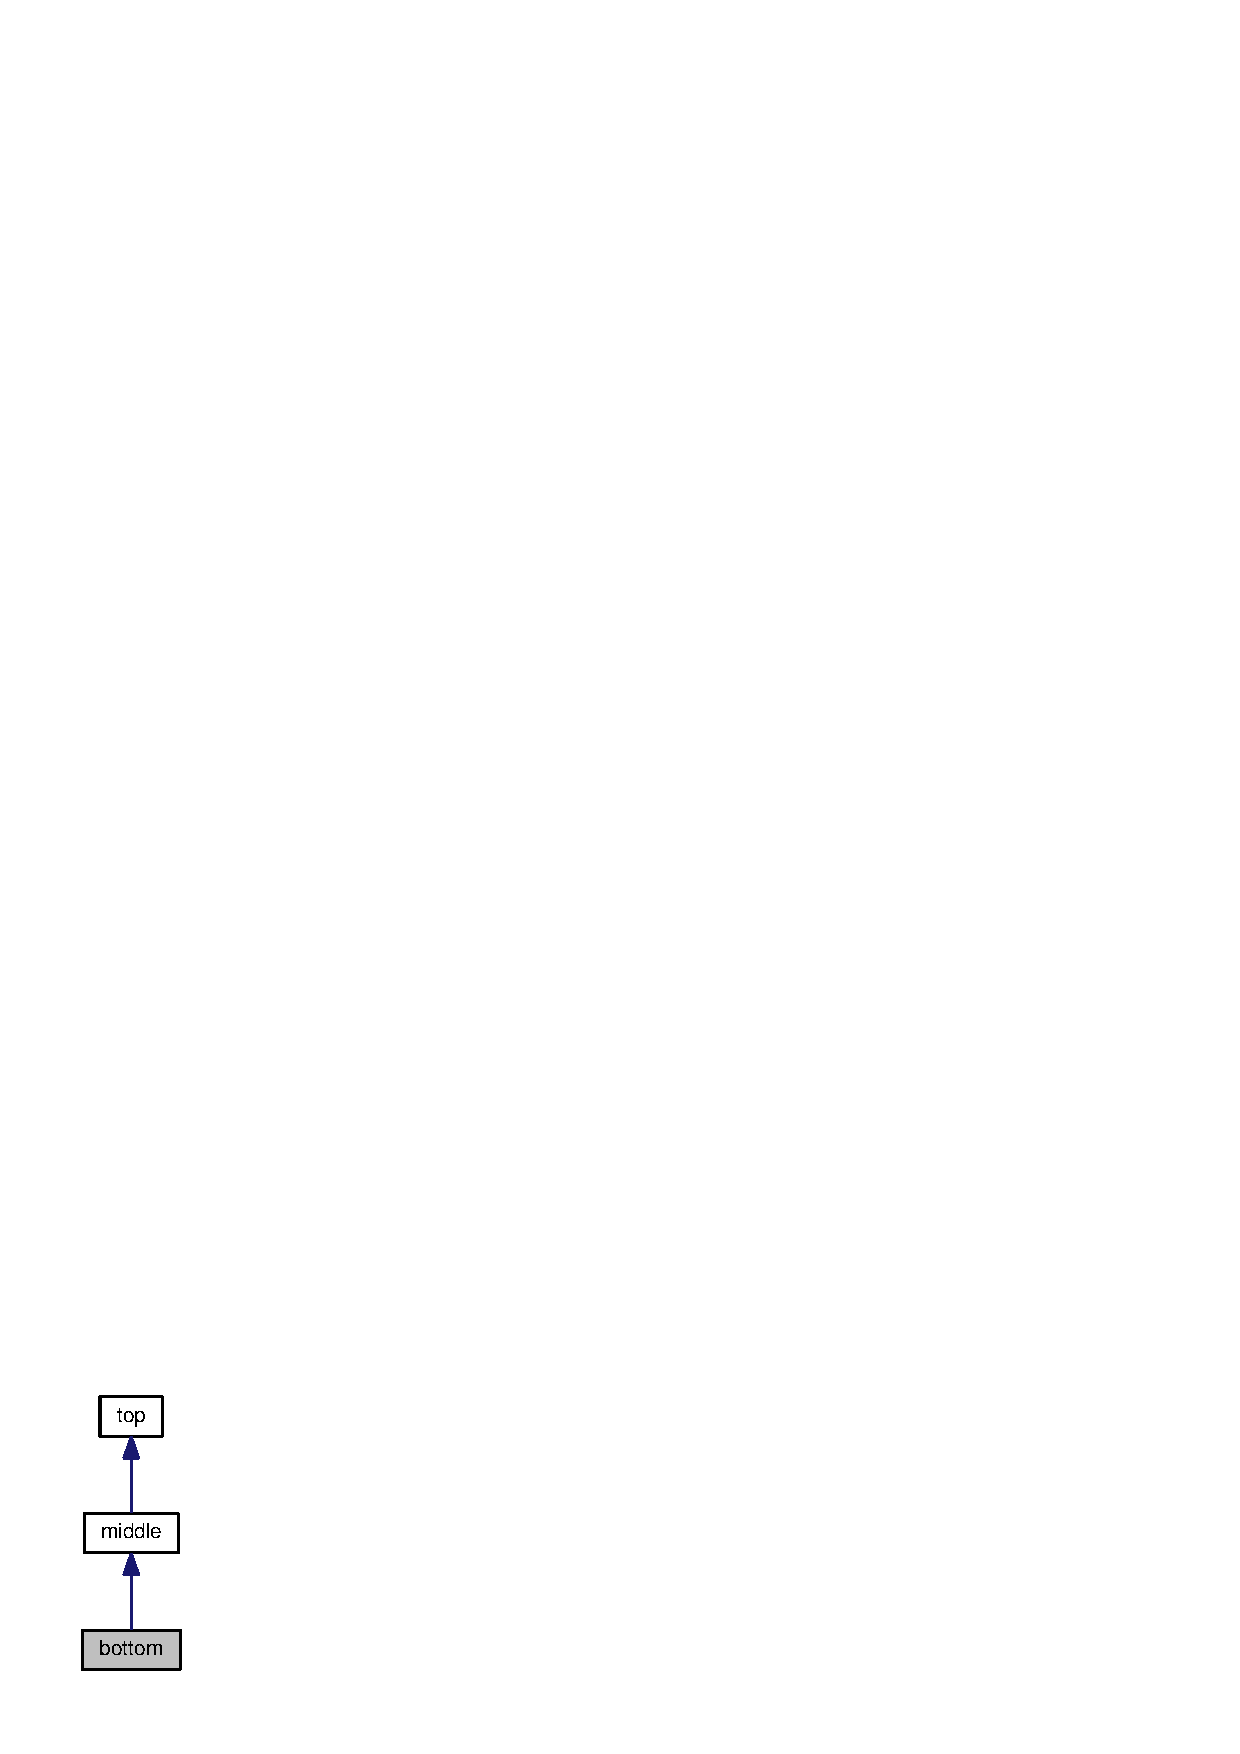
\includegraphics[width=90pt]{classbottom__inherit__graph}
\end{center}
\end{figure}


Collaboration diagram for bottom\-:\nopagebreak
\begin{figure}[H]
\begin{center}
\leavevmode
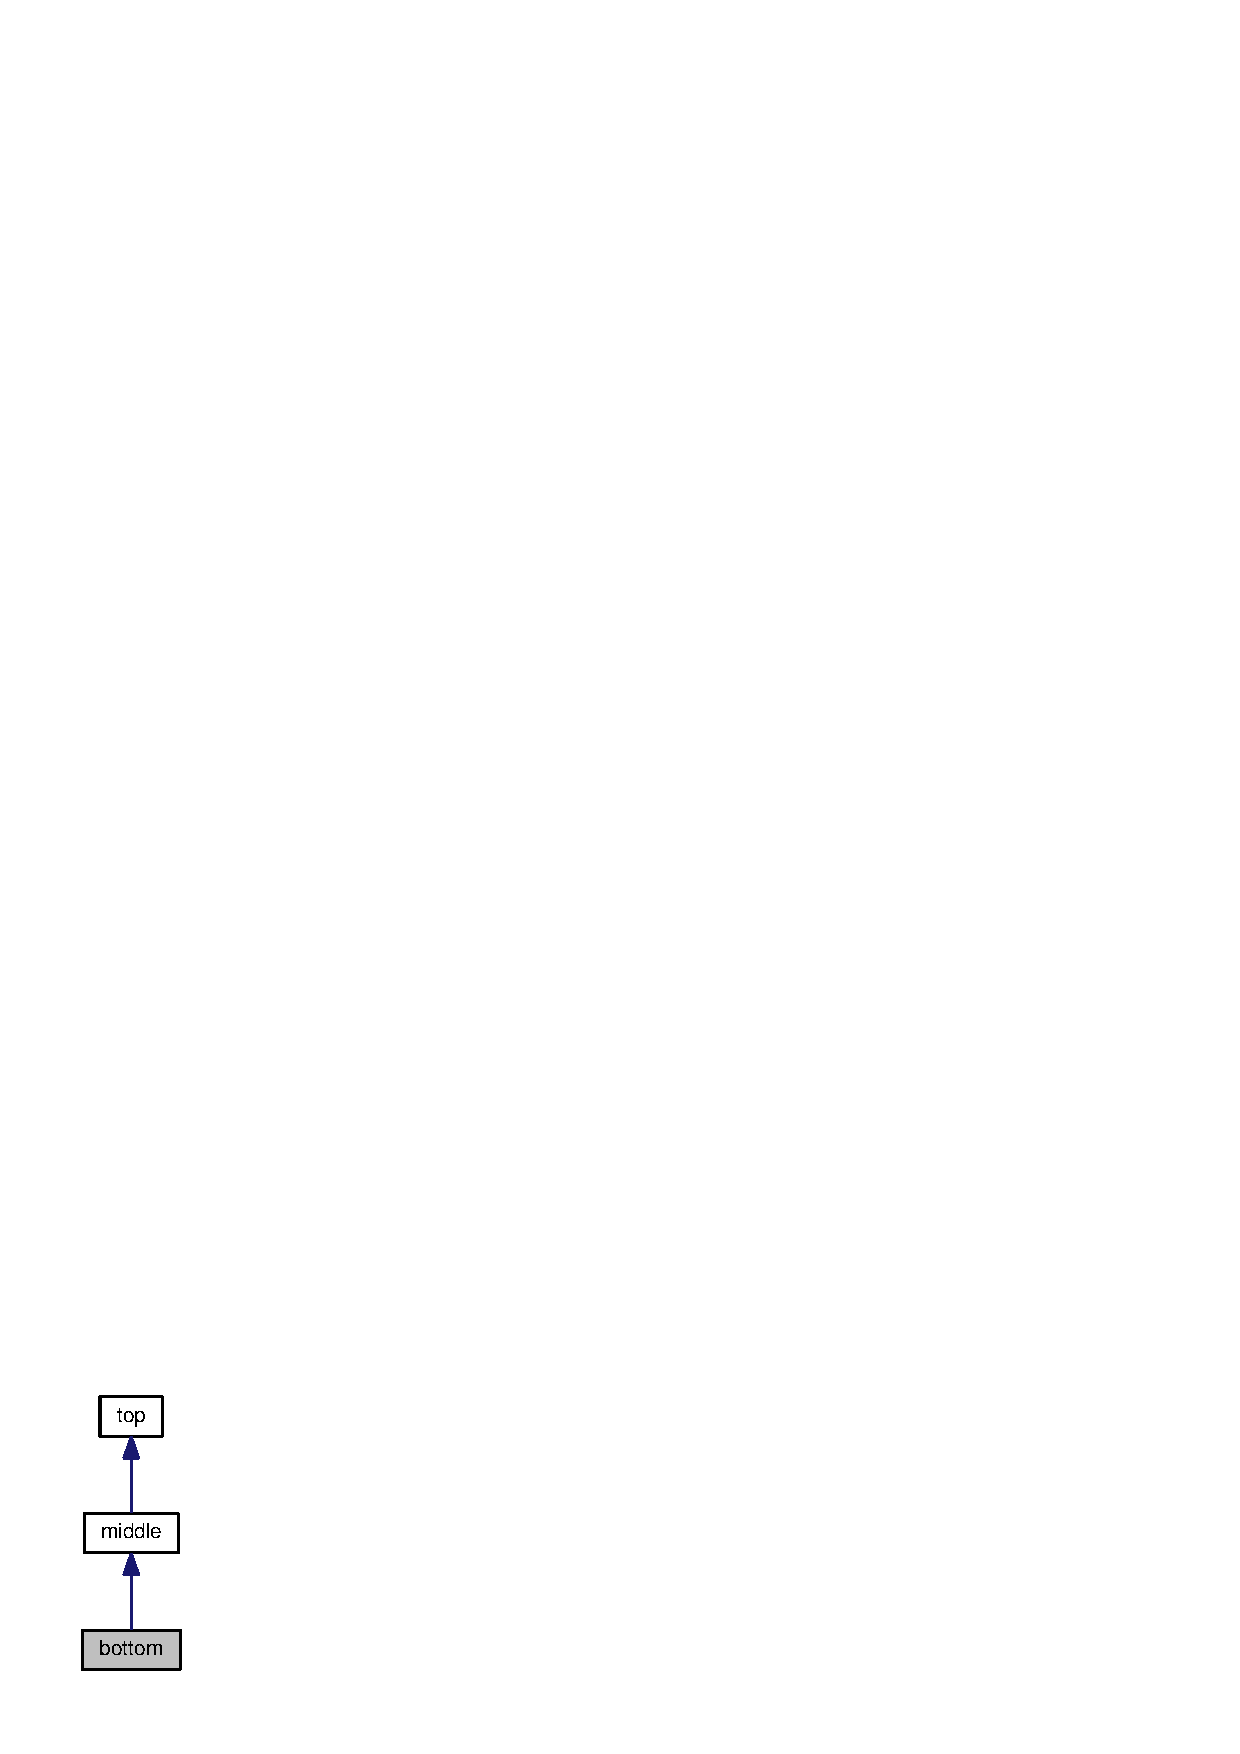
\includegraphics[width=90pt]{classbottom__coll__graph}
\end{center}
\end{figure}
\subsection*{Public Member Functions}
\begin{DoxyCompactItemize}
\item 
void {\bf cube} ()
\end{DoxyCompactItemize}
\subsection*{Public Attributes}
\begin{DoxyCompactItemize}
\item 
int {\bf c}
\end{DoxyCompactItemize}


\subsection{Detailed Description}


Definition at line 33 of file class.\-cc.



\subsection{Member Function Documentation}
\index{bottom@{bottom}!cube@{cube}}
\index{cube@{cube}!bottom@{bottom}}
\subsubsection[{cube}]{\setlength{\rightskip}{0pt plus 5cm}void bottom\-::cube (
\begin{DoxyParamCaption}
{}
\end{DoxyParamCaption}
)\hspace{0.3cm}{\ttfamily [inline]}}\label{classbottom_a6662ae9bde8fec3f306c54e1fb7b2ee6}


Definition at line 37 of file class.\-cc.



Referenced by main().


\begin{DoxyCode}
38 \{
39 square();
40 c=b*a;
41 cout<<\textcolor{stringliteral}{"\(\backslash\)n\(\backslash\)nCube :::\(\backslash\)t"}<<c;
42 \}
\end{DoxyCode}


Here is the caller graph for this function\-:\nopagebreak
\begin{figure}[H]
\begin{center}
\leavevmode
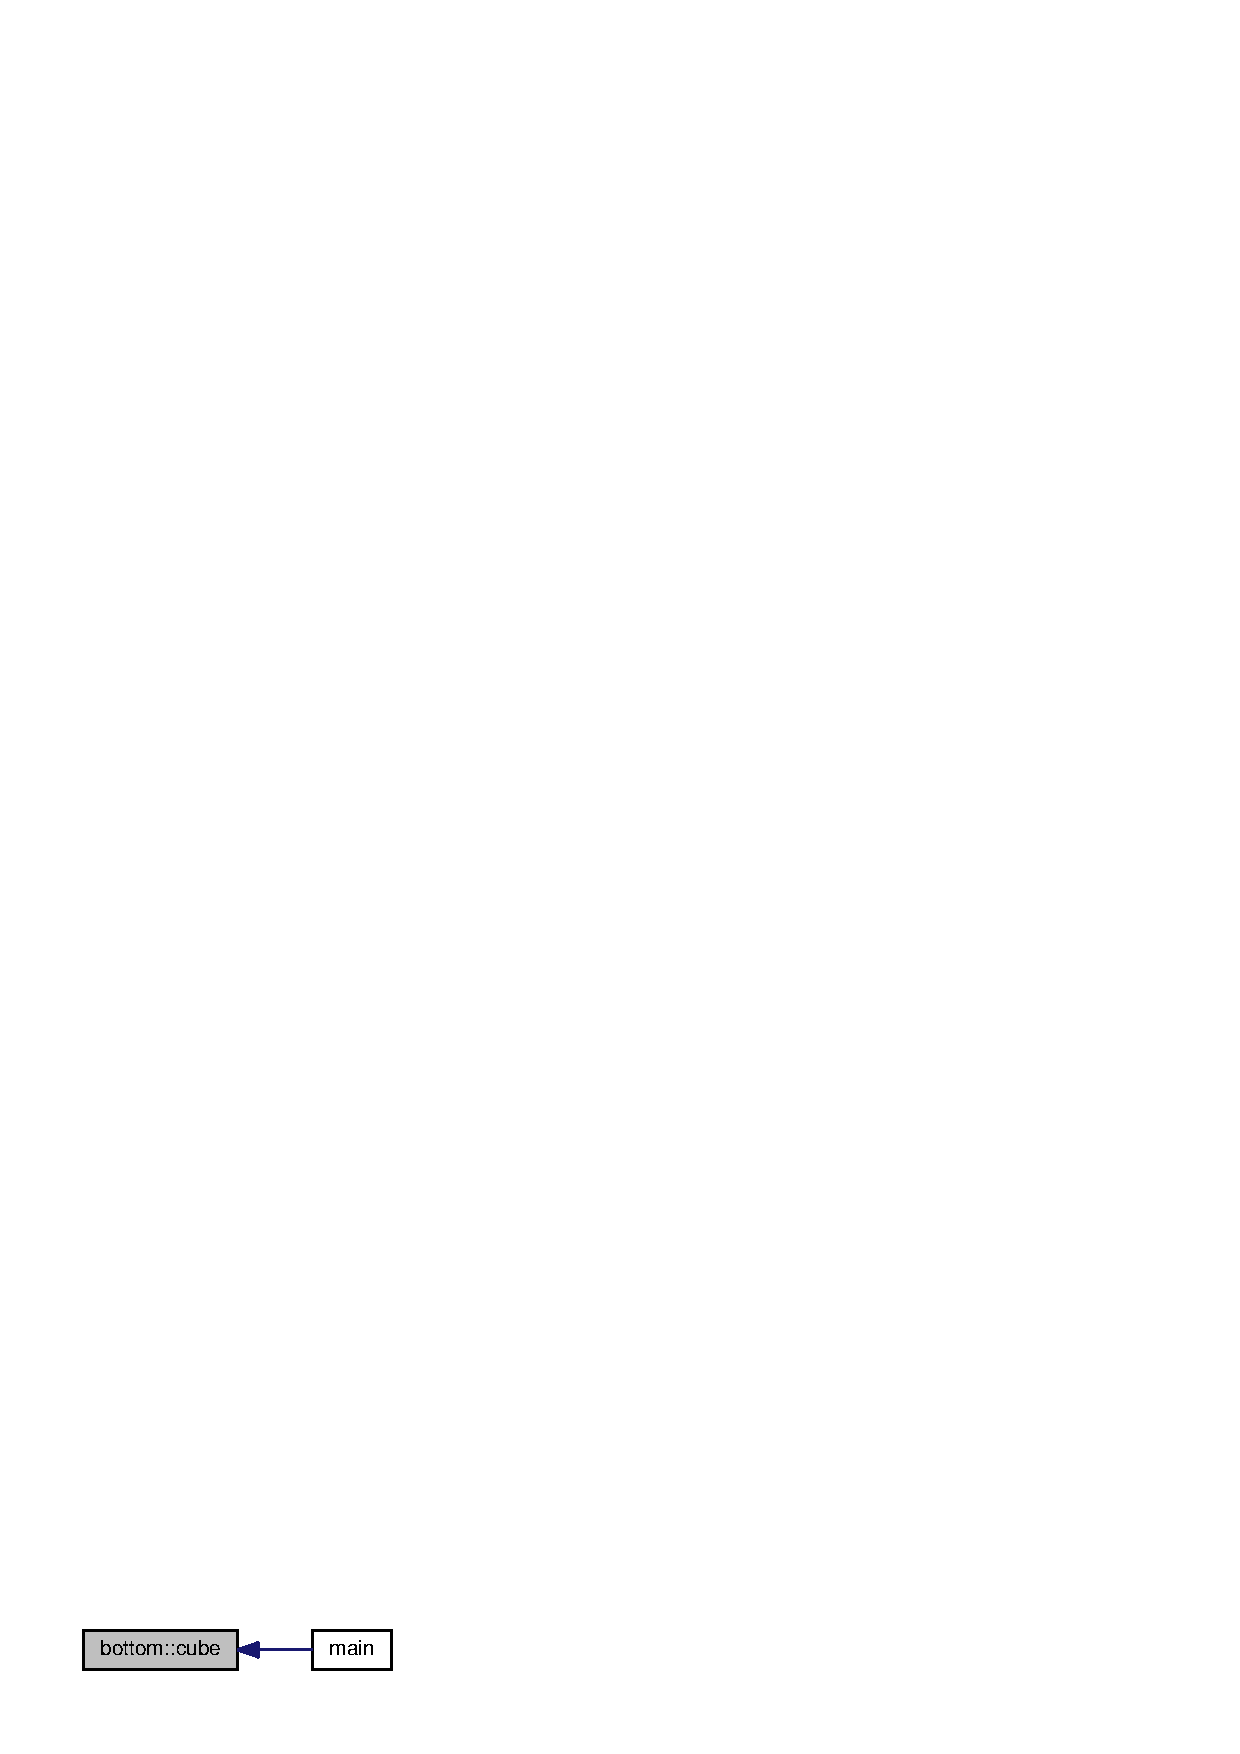
\includegraphics[width=192pt]{classbottom_a6662ae9bde8fec3f306c54e1fb7b2ee6_icgraph}
\end{center}
\end{figure}




\subsection{Member Data Documentation}
\index{bottom@{bottom}!c@{c}}
\index{c@{c}!bottom@{bottom}}
\subsubsection[{c}]{\setlength{\rightskip}{0pt plus 5cm}int bottom\-::c}\label{classbottom_a3a5c7cf54122860bcd8fc5ba5595d986}


Definition at line 36 of file class.\-cc.



The documentation for this class was generated from the following file\-:\begin{DoxyCompactItemize}
\item 
/home/manpreet/\-O\-C\-T\-A\-V\-E\-\_\-\-W\-O\-R\-K/{\bf class.\-cc}\end{DoxyCompactItemize}

\section{middle Class Reference}
\label{classmiddle}\index{middle@{middle}}


Inheritance diagram for middle\-:\nopagebreak
\begin{figure}[H]
\begin{center}
\leavevmode
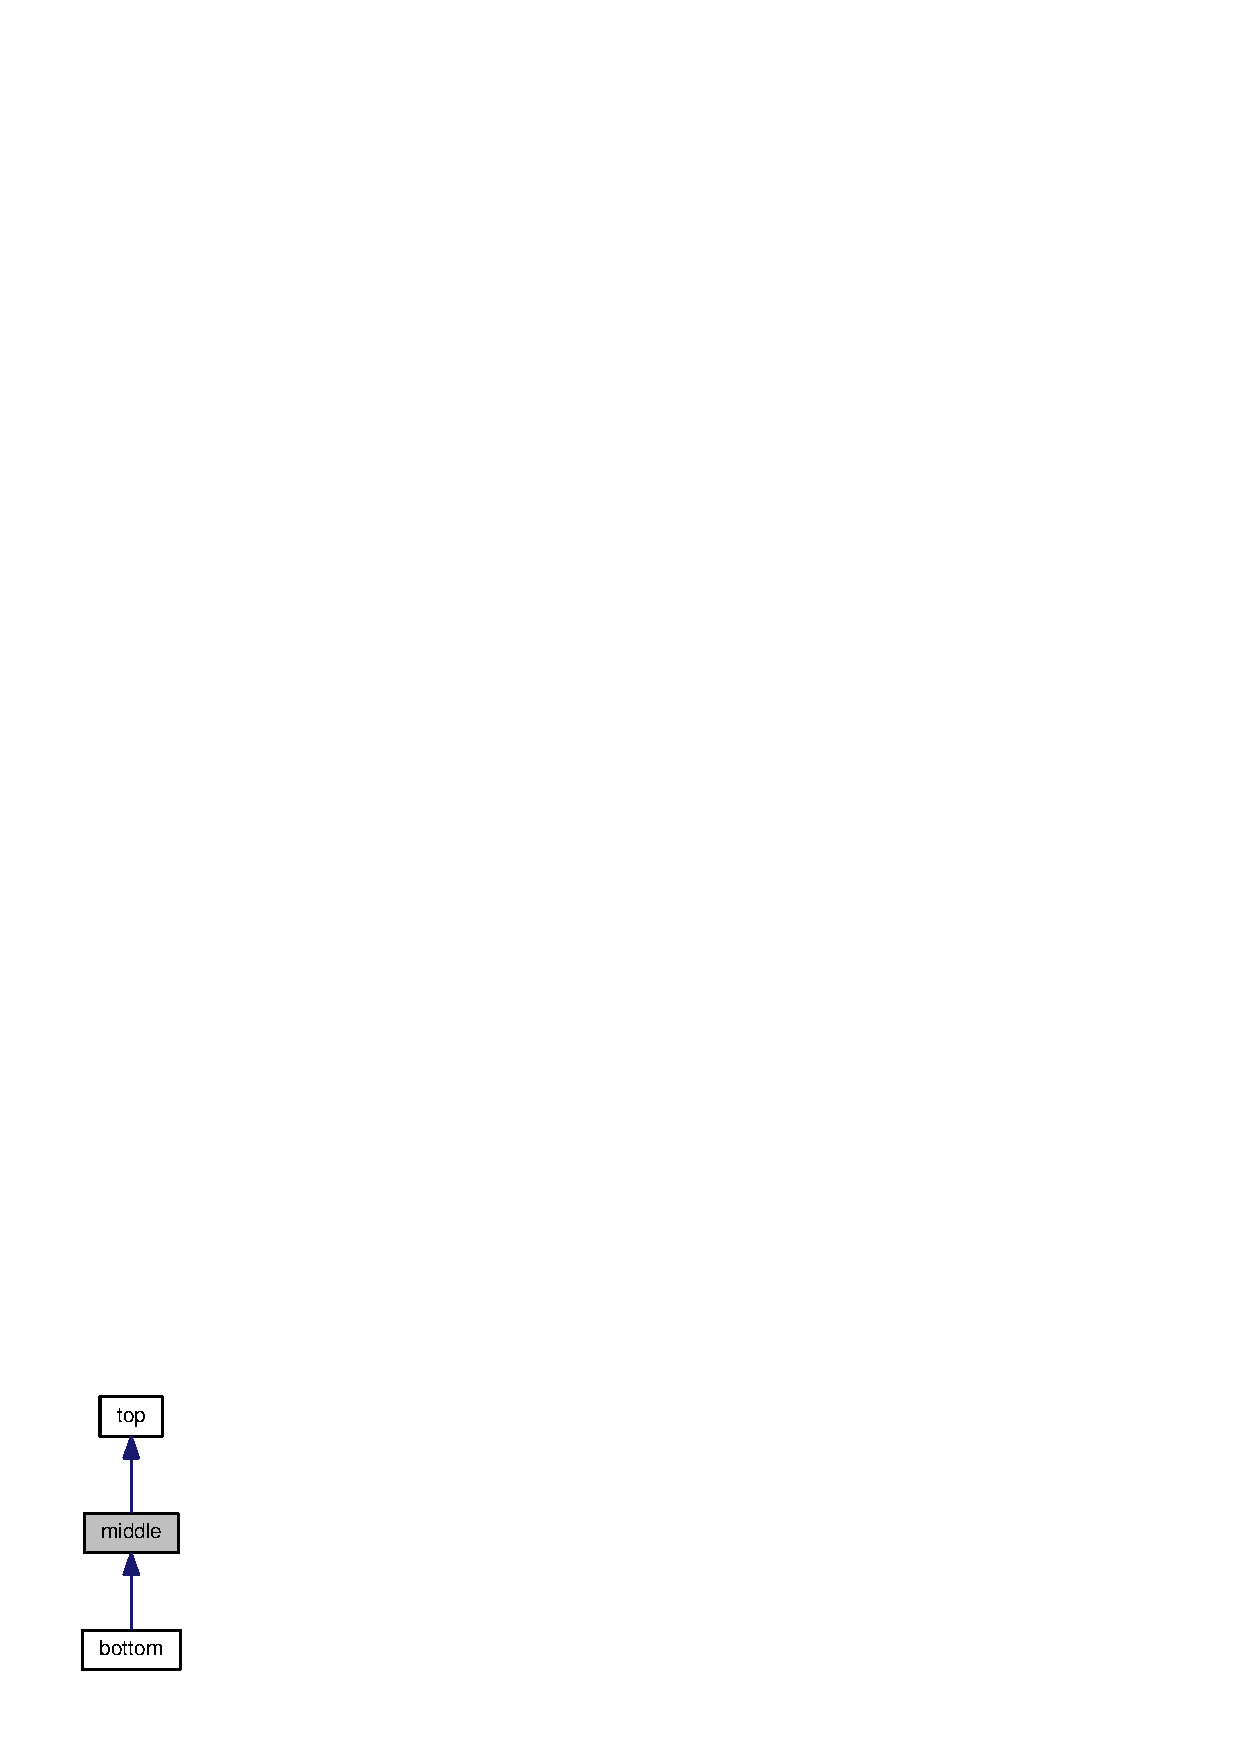
\includegraphics[width=90pt]{classmiddle__inherit__graph}
\end{center}
\end{figure}


Collaboration diagram for middle\-:\nopagebreak
\begin{figure}[H]
\begin{center}
\leavevmode
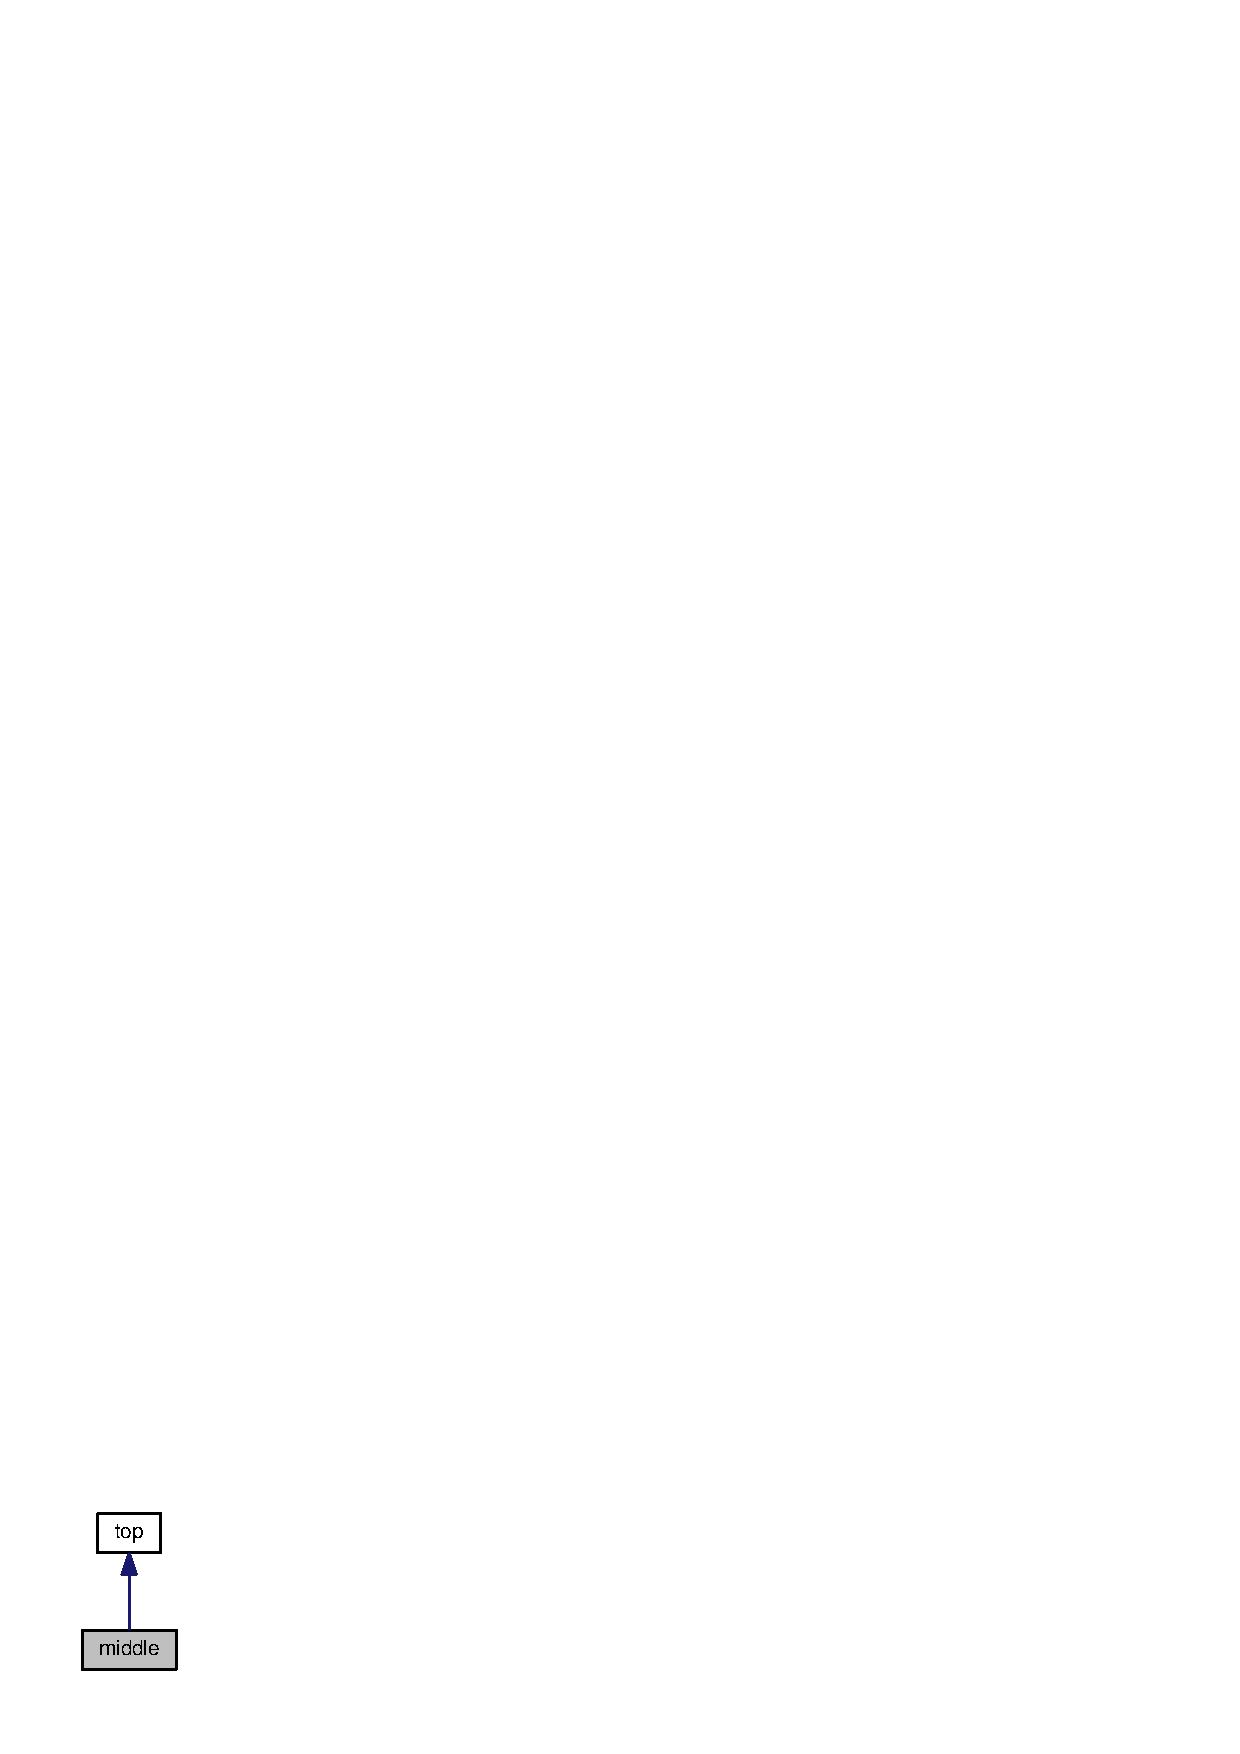
\includegraphics[width=88pt]{classmiddle__coll__graph}
\end{center}
\end{figure}
\subsection*{Public Member Functions}
\begin{DoxyCompactItemize}
\item 
void {\bf square} ()
\end{DoxyCompactItemize}
\subsection*{Public Attributes}
\begin{DoxyCompactItemize}
\item 
int {\bf b}
\end{DoxyCompactItemize}


\subsection{Detailed Description}


Definition at line 20 of file class.\-cc.



\subsection{Member Function Documentation}
\index{middle@{middle}!square@{square}}
\index{square@{square}!middle@{middle}}
\subsubsection[{square}]{\setlength{\rightskip}{0pt plus 5cm}void middle\-::square (
\begin{DoxyParamCaption}
{}
\end{DoxyParamCaption}
)\hspace{0.3cm}{\ttfamily [inline]}}\label{classmiddle_af99d979955a11660629f0e4d7f24d185}


Definition at line 24 of file class.\-cc.


\begin{DoxyCode}
25 \{
26 getdata();
27 b=a*a;
28 cout<<\textcolor{stringliteral}{"\(\backslash\)n\(\backslash\)nSquare Is :::"}<<b;
29 \}
\end{DoxyCode}


\subsection{Member Data Documentation}
\index{middle@{middle}!b@{b}}
\index{b@{b}!middle@{middle}}
\subsubsection[{b}]{\setlength{\rightskip}{0pt plus 5cm}int middle\-::b}\label{classmiddle_a368a6e9ee0176e14fcd0d24dca7d94ce}


Definition at line 23 of file class.\-cc.



The documentation for this class was generated from the following file\-:\begin{DoxyCompactItemize}
\item 
/home/manpreet/\-O\-C\-T\-A\-V\-E\-\_\-\-W\-O\-R\-K/{\bf class.\-cc}\end{DoxyCompactItemize}

\section{top Class Reference}
\label{classtop}\index{top@{top}}


Inheritance diagram for top\-:\nopagebreak
\begin{figure}[H]
\begin{center}
\leavevmode
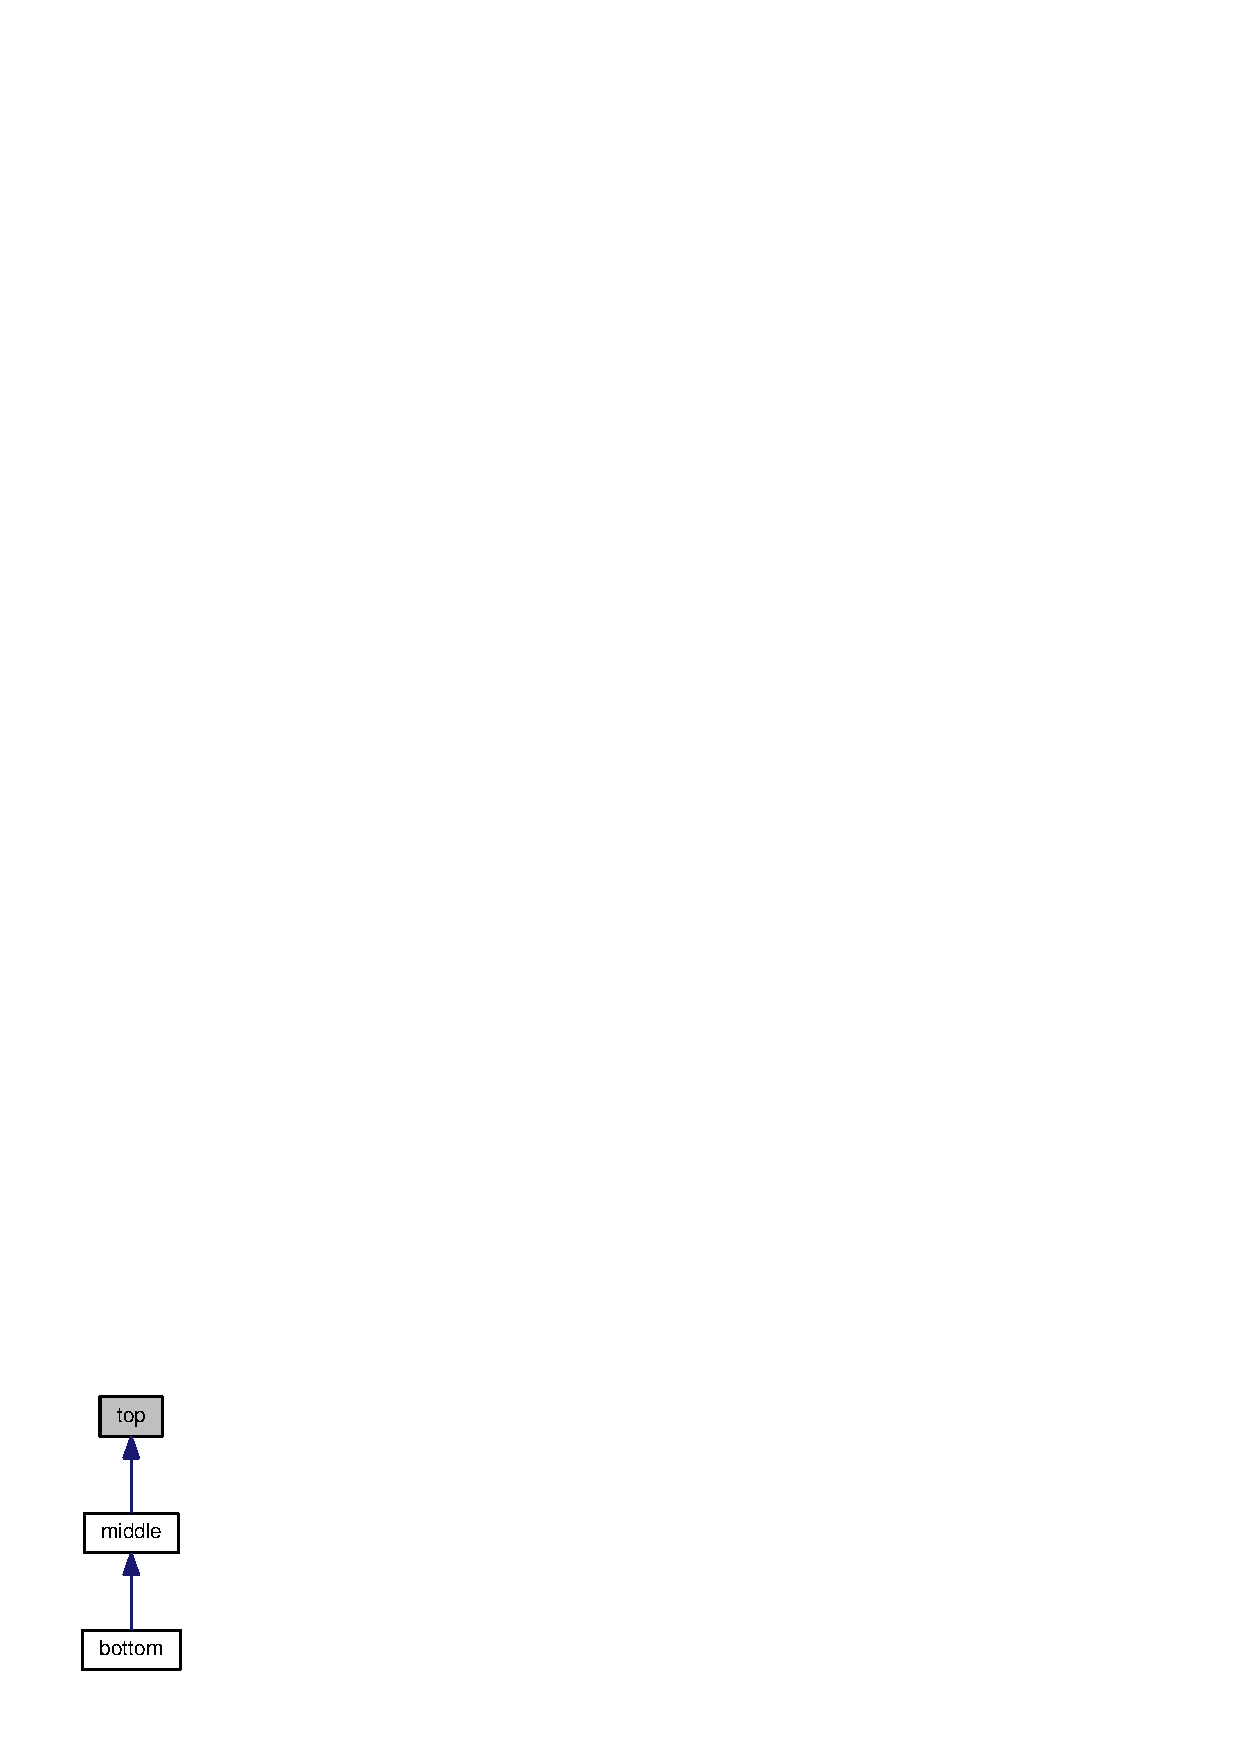
\includegraphics[width=90pt]{classtop__inherit__graph}
\end{center}
\end{figure}
\subsection*{Public Member Functions}
\begin{DoxyCompactItemize}
\item 
void {\bf getdata} ()
\item 
void {\bf putdata} ()
\end{DoxyCompactItemize}
\subsection*{Public Attributes}
\begin{DoxyCompactItemize}
\item 
int {\bf a}
\end{DoxyCompactItemize}


\subsection{Detailed Description}


Definition at line 4 of file class.\-cc.



\subsection{Member Function Documentation}
\index{top@{top}!getdata@{getdata}}
\index{getdata@{getdata}!top@{top}}
\subsubsection[{getdata}]{\setlength{\rightskip}{0pt plus 5cm}void top\-::getdata (
\begin{DoxyParamCaption}
{}
\end{DoxyParamCaption}
)\hspace{0.3cm}{\ttfamily [inline]}}\label{classtop_a2b95f14d671ea868ac7e77e163b4fcce}


Definition at line 8 of file class.\-cc.



Referenced by main().


\begin{DoxyCode}
9 \{
10 cout<<\textcolor{stringliteral}{"\(\backslash\)n\(\backslash\)nEnter first Number :::\(\backslash\)t"};
11 cin>>a;
12 \}
\end{DoxyCode}


Here is the caller graph for this function\-:\nopagebreak
\begin{figure}[H]
\begin{center}
\leavevmode
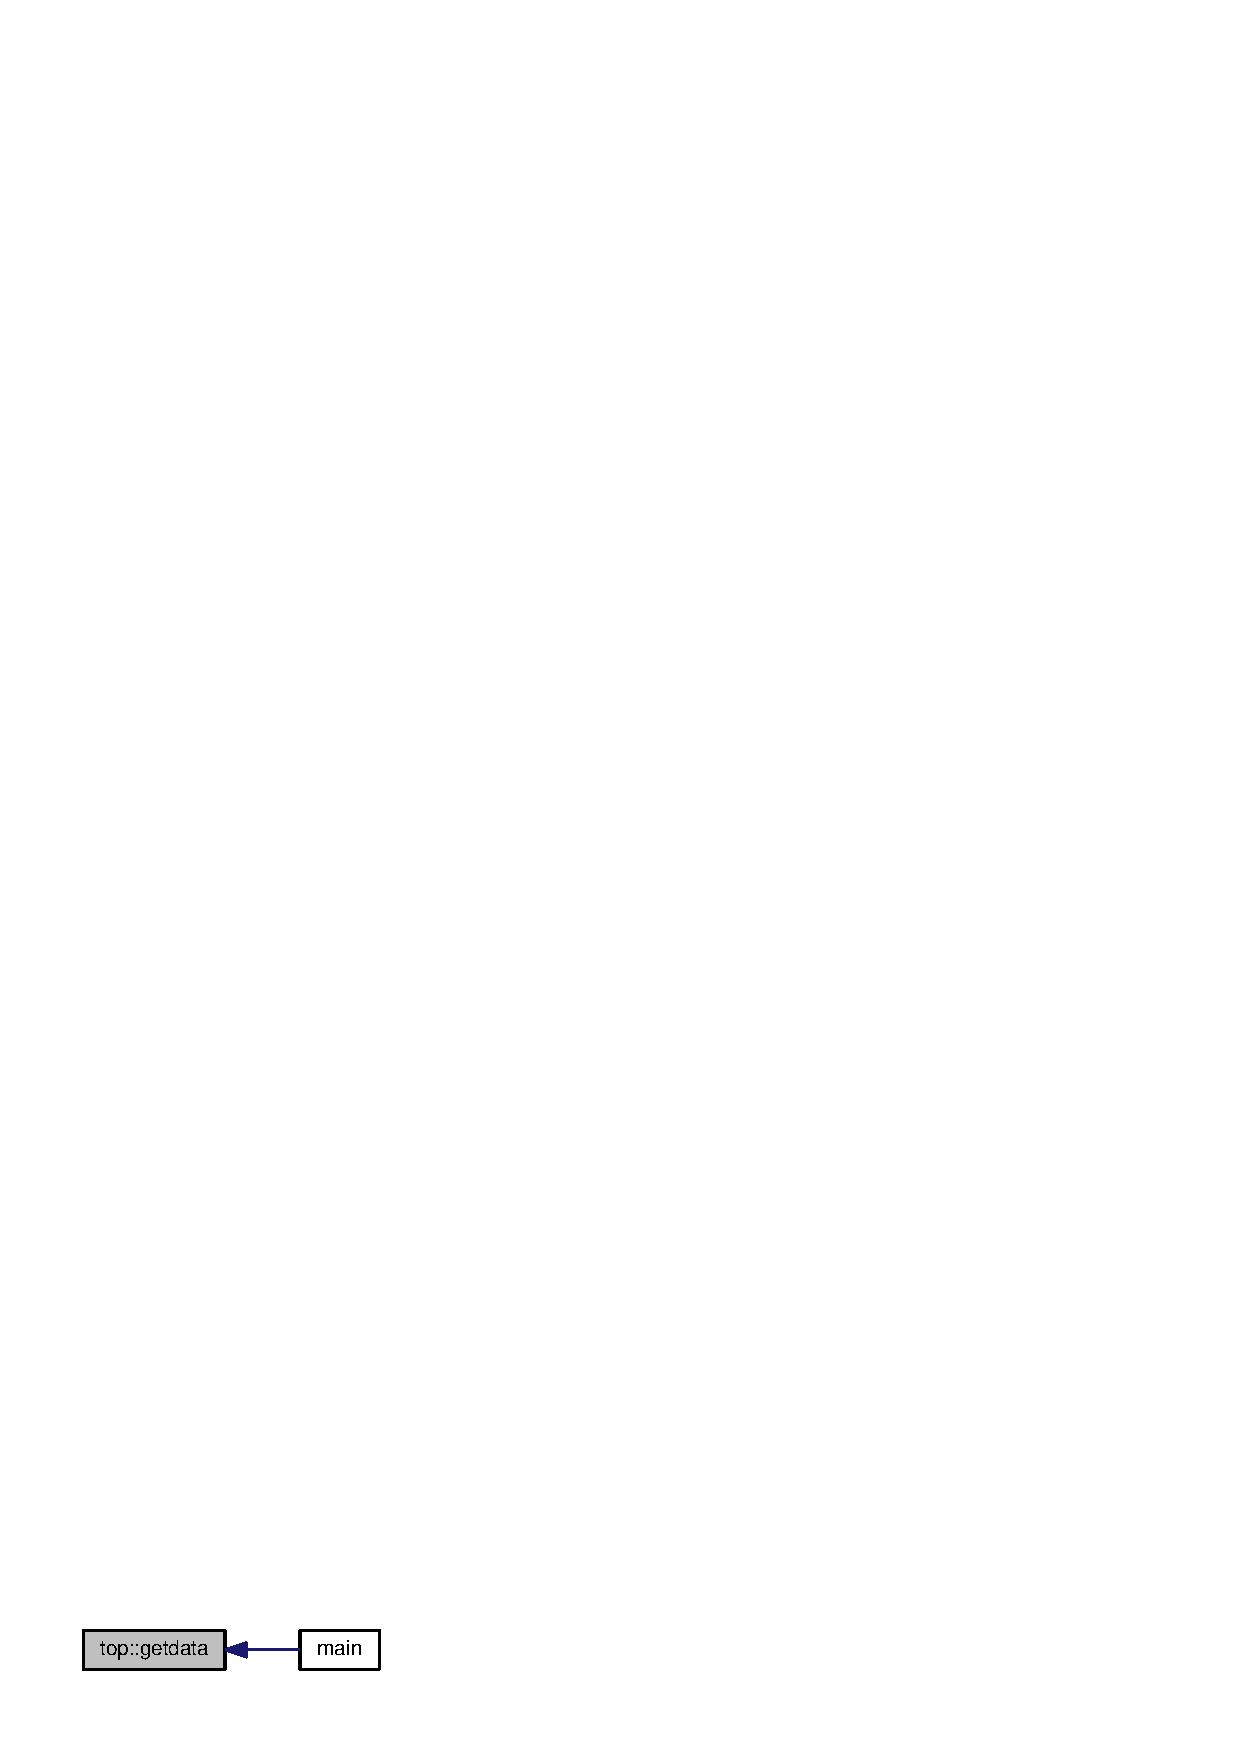
\includegraphics[width=186pt]{classtop_a2b95f14d671ea868ac7e77e163b4fcce_icgraph}
\end{center}
\end{figure}


\index{top@{top}!putdata@{putdata}}
\index{putdata@{putdata}!top@{top}}
\subsubsection[{putdata}]{\setlength{\rightskip}{0pt plus 5cm}void top\-::putdata (
\begin{DoxyParamCaption}
{}
\end{DoxyParamCaption}
)\hspace{0.3cm}{\ttfamily [inline]}}\label{classtop_a422bc856443aa1975c74122d6ed59b70}


Definition at line 13 of file class.\-cc.



Referenced by main().


\begin{DoxyCode}
14 \{
15 cout<<\textcolor{stringliteral}{"\(\backslash\)nFirst Number Is :::\(\backslash\)t"}<<a;
16 \}
\end{DoxyCode}


Here is the caller graph for this function\-:\nopagebreak
\begin{figure}[H]
\begin{center}
\leavevmode
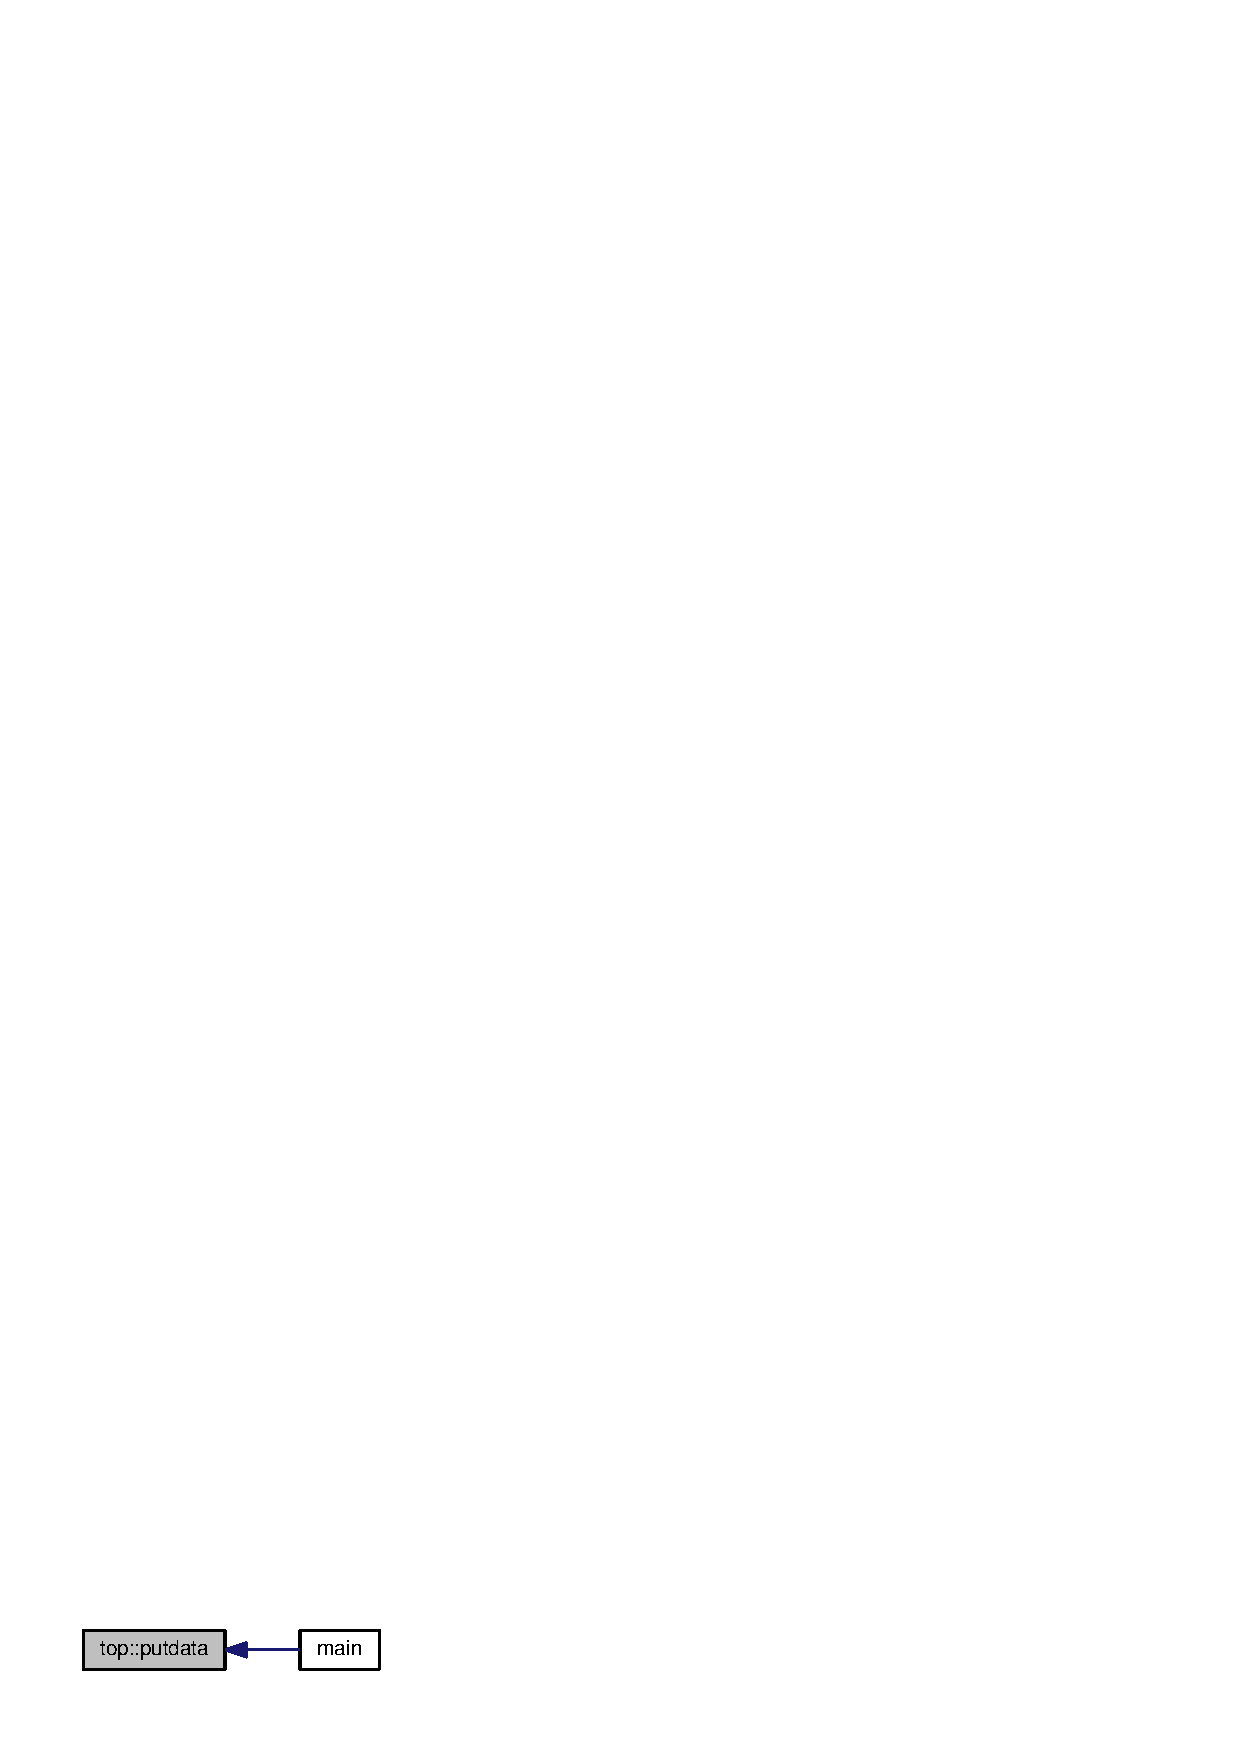
\includegraphics[width=186pt]{classtop_a422bc856443aa1975c74122d6ed59b70_icgraph}
\end{center}
\end{figure}




\subsection{Member Data Documentation}
\index{top@{top}!a@{a}}
\index{a@{a}!top@{top}}
\subsubsection[{a}]{\setlength{\rightskip}{0pt plus 5cm}int top\-::a}\label{classtop_a872b030cc6806bd91642f26dd3cd6050}


Definition at line 7 of file class.\-cc.



The documentation for this class was generated from the following file\-:\begin{DoxyCompactItemize}
\item 
/home/manpreet/\-O\-C\-T\-A\-V\-E\-\_\-\-W\-O\-R\-K/{\bf class.\-cc}\end{DoxyCompactItemize}

\chapter{File Documentation}
\section{/home/manpreet/\-O\-C\-T\-A\-V\-E\-\_\-\-W\-O\-R\-K/civil.m File Reference}
\label{civil_8m}\index{/home/manpreet/\-O\-C\-T\-A\-V\-E\-\_\-\-W\-O\-R\-K/civil.\-m@{/home/manpreet/\-O\-C\-T\-A\-V\-E\-\_\-\-W\-O\-R\-K/civil.\-m}}
\subsection*{Functions}
\begin{DoxyCompactItemize}
\item 
otherwise {\bf warning} ('Unexpected soil type') end {\bf if}(time\-Prd$<$ {\bf t2}) {\bf sag}
\item 
{\bf elseif} (time\-Prd $>$ {\bf t3}) {\bf sag}
\item 
end end {\bf function} {\bf matrix\-Te\-X} ({\bf A}, fmt, align) disp(['\textbackslash{}section
\end{DoxyCompactItemize}
\subsection*{Variables}
\begin{DoxyCompactItemize}
\item 
calculate global stiffness \\*
matrix {\bf clc} {\bf clear} load input \\*
mat Soil\-\_\-type {\bf Type\-\_\-of\-\_\-soil} = ''
\item 
for {\bf i}
\item 
end {\bf Type\-\_\-of\-\_\-soil} Function to \\*
write Matrix {\bf t1} = 0
\item 
{\bf t2} = 0
\item 
{\bf t3} = 0
\item 
{\bf t4} = 0
\item 
{\bf eq3num} = 0
\item 
{\bf function} {\bf sag}
\end{DoxyCompactItemize}


\subsection{Function Documentation}
\index{civil.\-m@{civil.\-m}!elseif@{elseif}}
\index{elseif@{elseif}!civil.m@{civil.\-m}}
\subsubsection[{elseif}]{\setlength{\rightskip}{0pt plus 5cm}elseif (
\begin{DoxyParamCaption}
\item[{time\-Prd}]{, }
\item[{{\bf t3}}]{}
\end{DoxyParamCaption}
)}\label{civil_8m_a0d135864d9bc0103cbd903c62d64b088}
\index{civil.\-m@{civil.\-m}!matrix\-Te\-X@{matrix\-Te\-X}}
\index{matrix\-Te\-X@{matrix\-Te\-X}!civil.m@{civil.\-m}}
\subsubsection[{matrix\-Te\-X}]{\setlength{\rightskip}{0pt plus 5cm}end end {\bf function} matrix\-Te\-X (
\begin{DoxyParamCaption}
\item[{{\bf A}}]{, }
\item[{fmt}]{, }
\item[{align}]{}
\end{DoxyParamCaption}
)}\label{civil_8m_a8c0a4f44ca03289871d3743578e0412c}


Definition at line 43 of file civil.\-m.

\index{civil.\-m@{civil.\-m}!warning@{warning}}
\index{warning@{warning}!civil.m@{civil.\-m}}
\subsubsection[{warning}]{\setlength{\rightskip}{0pt plus 5cm}otherwise warning (
\begin{DoxyParamCaption}
\item[{'Unexpected soil type'}]{}
\end{DoxyParamCaption}
)}\label{civil_8m_a29249d852e6e3fd1e206e1f920300e24}


\subsection{Variable Documentation}
\index{civil.\-m@{civil.\-m}!eq3num@{eq3num}}
\index{eq3num@{eq3num}!civil.m@{civil.\-m}}
\subsubsection[{eq3num}]{\setlength{\rightskip}{0pt plus 5cm}eq3num = 0}\label{civil_8m_a8ecbd124ddcdab7fc367443a82b241af}


Definition at line 20 of file civil.\-m.

\index{civil.\-m@{civil.\-m}!i@{i}}
\index{i@{i}!civil.m@{civil.\-m}}
\subsubsection[{i}]{\setlength{\rightskip}{0pt plus 5cm}for i}\label{civil_8m_a6f6ccfcf58b31cb6412107d9d5281426}
{\bfseries Initial value\-:}
\begin{DoxyCode}
= 1:Soil\_type
  Type_of_soil = strcat(Type_of_soil, \textcolor{charliteral}{'I'})
\end{DoxyCode}


Definition at line 11 of file civil.\-m.



Referenced by main().

\index{civil.\-m@{civil.\-m}!sag@{sag}}
\index{sag@{sag}!civil.m@{civil.\-m}}
\subsubsection[{sag}]{\setlength{\rightskip}{0pt plus 5cm}else sag}\label{civil_8m_aac9abc95cd2ddc27fa84fb4440b62888}
{\bfseries Initial value\-:}
\begin{DoxyCode}
= funSaog(soilType, timePrd)
  t2 = 0.10
\end{DoxyCode}


Definition at line 22 of file civil.\-m.

\index{civil.\-m@{civil.\-m}!t1@{t1}}
\index{t1@{t1}!civil.m@{civil.\-m}}
\subsubsection[{t1}]{\setlength{\rightskip}{0pt plus 5cm}end {\bf Type\-\_\-of\-\_\-soil} Function to write Matrix t1 = 0}\label{civil_8m_a3a318718cf4c9c1380475d059171d8f3}


Definition at line 19 of file civil.\-m.

\index{civil.\-m@{civil.\-m}!t2@{t2}}
\index{t2@{t2}!civil.m@{civil.\-m}}
\subsubsection[{t2}]{\setlength{\rightskip}{0pt plus 5cm}t2 = 0}\label{civil_8m_a24aeadb733f27244ec14e4cba82eeee9}


Definition at line 19 of file civil.\-m.

\index{civil.\-m@{civil.\-m}!t3@{t3}}
\index{t3@{t3}!civil.m@{civil.\-m}}
\subsubsection[{t3}]{\setlength{\rightskip}{0pt plus 5cm}case I\-I\-I t3 = 0}\label{civil_8m_a80d62394ff82e3ae283e9113bca340a2}


Definition at line 19 of file civil.\-m.

\index{civil.\-m@{civil.\-m}!t4@{t4}}
\index{t4@{t4}!civil.m@{civil.\-m}}
\subsubsection[{t4}]{\setlength{\rightskip}{0pt plus 5cm}t4 = 0}\label{civil_8m_ae95ab11d59379638967673bd74654b2a}


Definition at line 19 of file civil.\-m.

\index{civil.\-m@{civil.\-m}!Type\-\_\-of\-\_\-soil@{Type\-\_\-of\-\_\-soil}}
\index{Type\-\_\-of\-\_\-soil@{Type\-\_\-of\-\_\-soil}!civil.m@{civil.\-m}}
\subsubsection[{Type\-\_\-of\-\_\-soil}]{\setlength{\rightskip}{0pt plus 5cm}calculate global stiffness matrix {\bf clc} {\bf clear} load input mat Soil\-\_\-type Type\-\_\-of\-\_\-soil = ''}\label{civil_8m_ac99038f2b9e5cc7205903d742faffd30}


Definition at line 9 of file civil.\-m.


\section{/home/manpreet/\-O\-C\-T\-A\-V\-E\-\_\-\-W\-O\-R\-K/class.cc File Reference}
\label{class_8cc}\index{/home/manpreet/\-O\-C\-T\-A\-V\-E\-\_\-\-W\-O\-R\-K/class.\-cc@{/home/manpreet/\-O\-C\-T\-A\-V\-E\-\_\-\-W\-O\-R\-K/class.\-cc}}
{\ttfamily \#include $<$iostream$>$}\\*
Include dependency graph for class.\-cc\-:\nopagebreak
\begin{figure}[H]
\begin{center}
\leavevmode
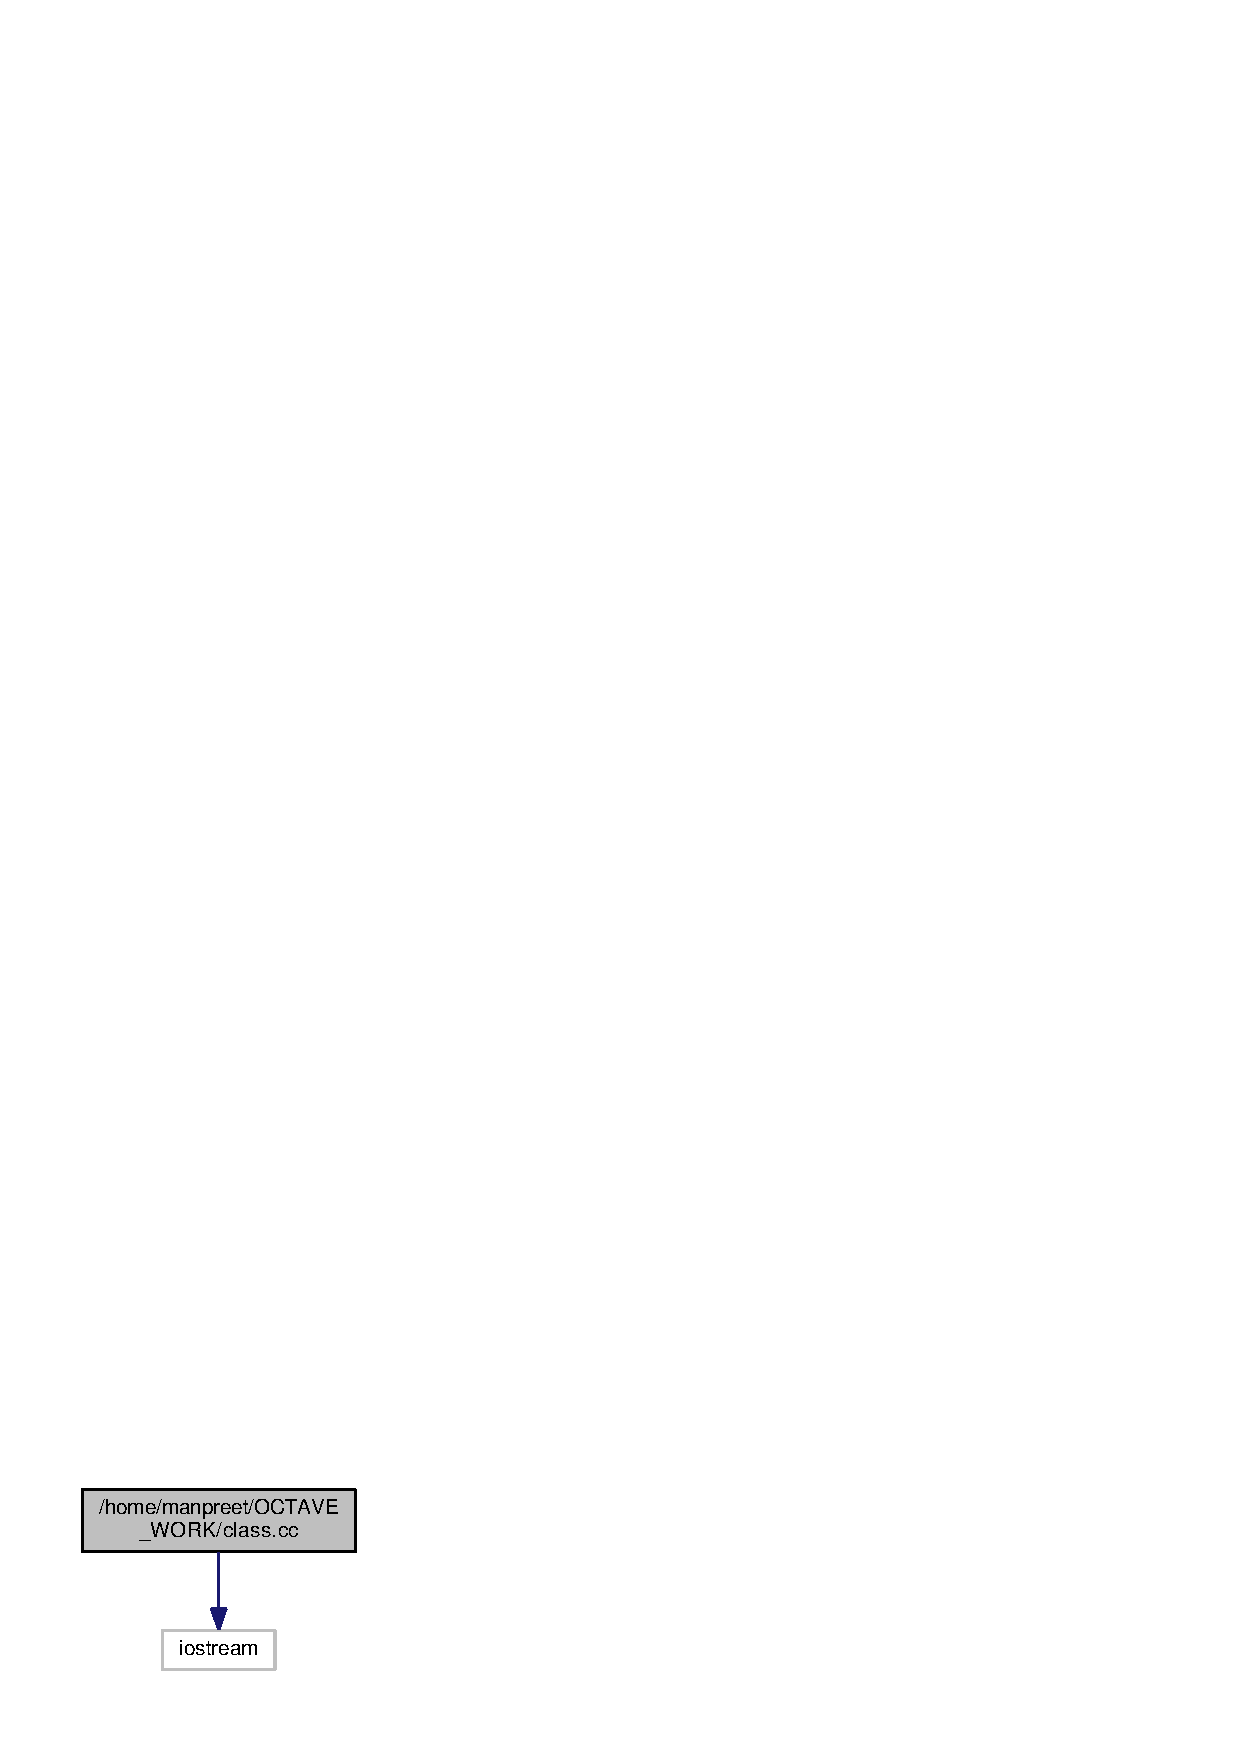
\includegraphics[width=174pt]{class_8cc__incl}
\end{center}
\end{figure}
\subsection*{Classes}
\begin{DoxyCompactItemize}
\item 
class {\bf top}
\item 
class {\bf middle}
\item 
class {\bf bottom}
\end{DoxyCompactItemize}
\subsection*{Functions}
\begin{DoxyCompactItemize}
\item 
int {\bf main} ()
\end{DoxyCompactItemize}


\subsection{Function Documentation}
\index{class.\-cc@{class.\-cc}!main@{main}}
\index{main@{main}!class.cc@{class.\-cc}}
\subsubsection[{main}]{\setlength{\rightskip}{0pt plus 5cm}int main (
\begin{DoxyParamCaption}
{}
\end{DoxyParamCaption}
)}\label{class_8cc_ae66f6b31b5ad750f1fe042a706a4e3d4}


Definition at line 45 of file class.\-cc.



References bottom\-::cube(), top\-::getdata(), and top\-::putdata().


\begin{DoxyCode}
46 \{
47 \textcolor{comment}{//clrscr();}
48 bottom b1;
49 b1.getdata();
50 b1.cube();
51 b1.putdata();
52 \textcolor{keywordflow}{return} 0;
53 \}
\end{DoxyCode}


Here is the call graph for this function\-:\nopagebreak
\begin{figure}[H]
\begin{center}
\leavevmode
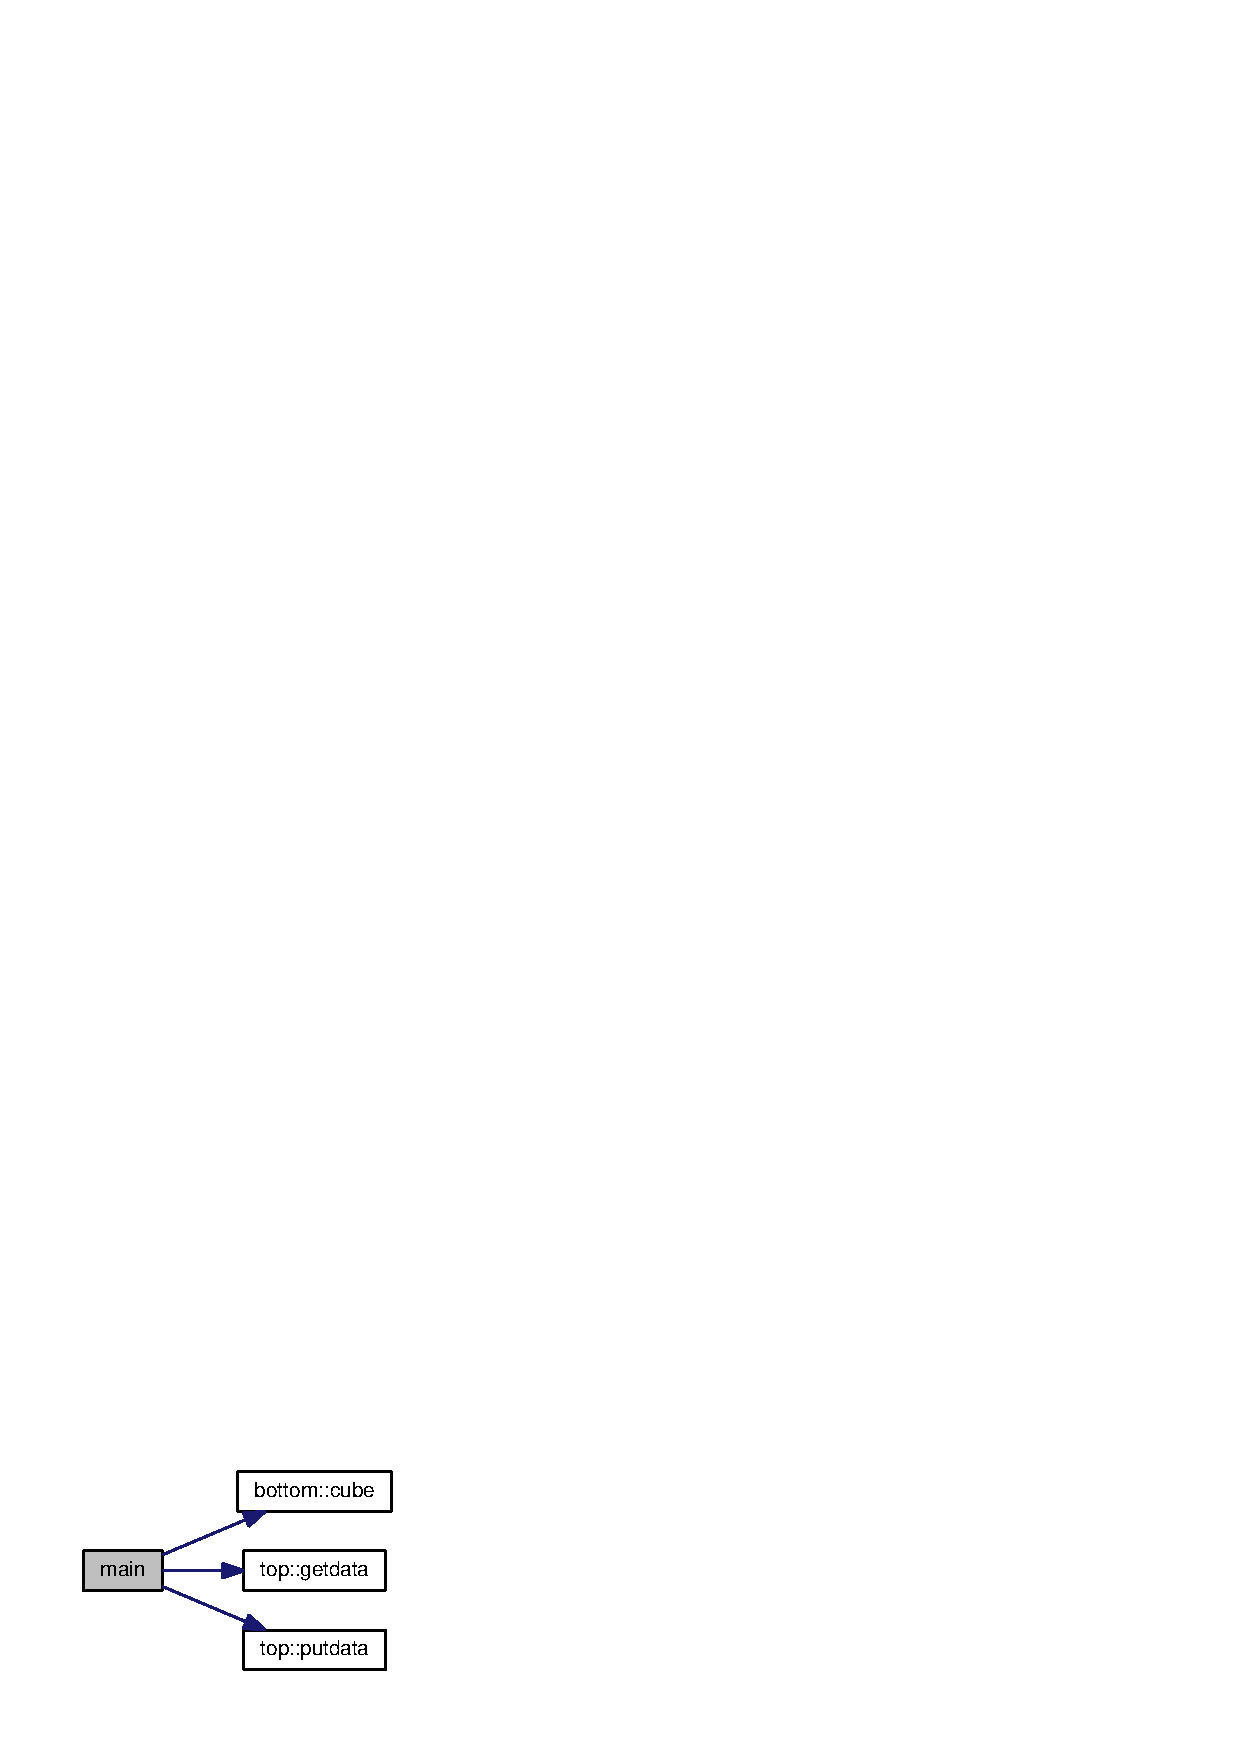
\includegraphics[width=192pt]{class_8cc_ae66f6b31b5ad750f1fe042a706a4e3d4_cgraph}
\end{center}
\end{figure}



\section{/home/manpreet/\-O\-C\-T\-A\-V\-E\-\_\-\-W\-O\-R\-K/d.cc File Reference}
\label{d_8cc}\index{/home/manpreet/\-O\-C\-T\-A\-V\-E\-\_\-\-W\-O\-R\-K/d.\-cc@{/home/manpreet/\-O\-C\-T\-A\-V\-E\-\_\-\-W\-O\-R\-K/d.\-cc}}

\section{/home/manpreet/\-O\-C\-T\-A\-V\-E\-\_\-\-W\-O\-R\-K/de.cc File Reference}
\label{de_8cc}\index{/home/manpreet/\-O\-C\-T\-A\-V\-E\-\_\-\-W\-O\-R\-K/de.\-cc@{/home/manpreet/\-O\-C\-T\-A\-V\-E\-\_\-\-W\-O\-R\-K/de.\-cc}}
{\ttfamily \#include $<$iostream$>$}\\*
{\ttfamily \#include $<$octave/oct.\-h$>$}\\*
Include dependency graph for de.\-cc\-:\nopagebreak
\begin{figure}[H]
\begin{center}
\leavevmode
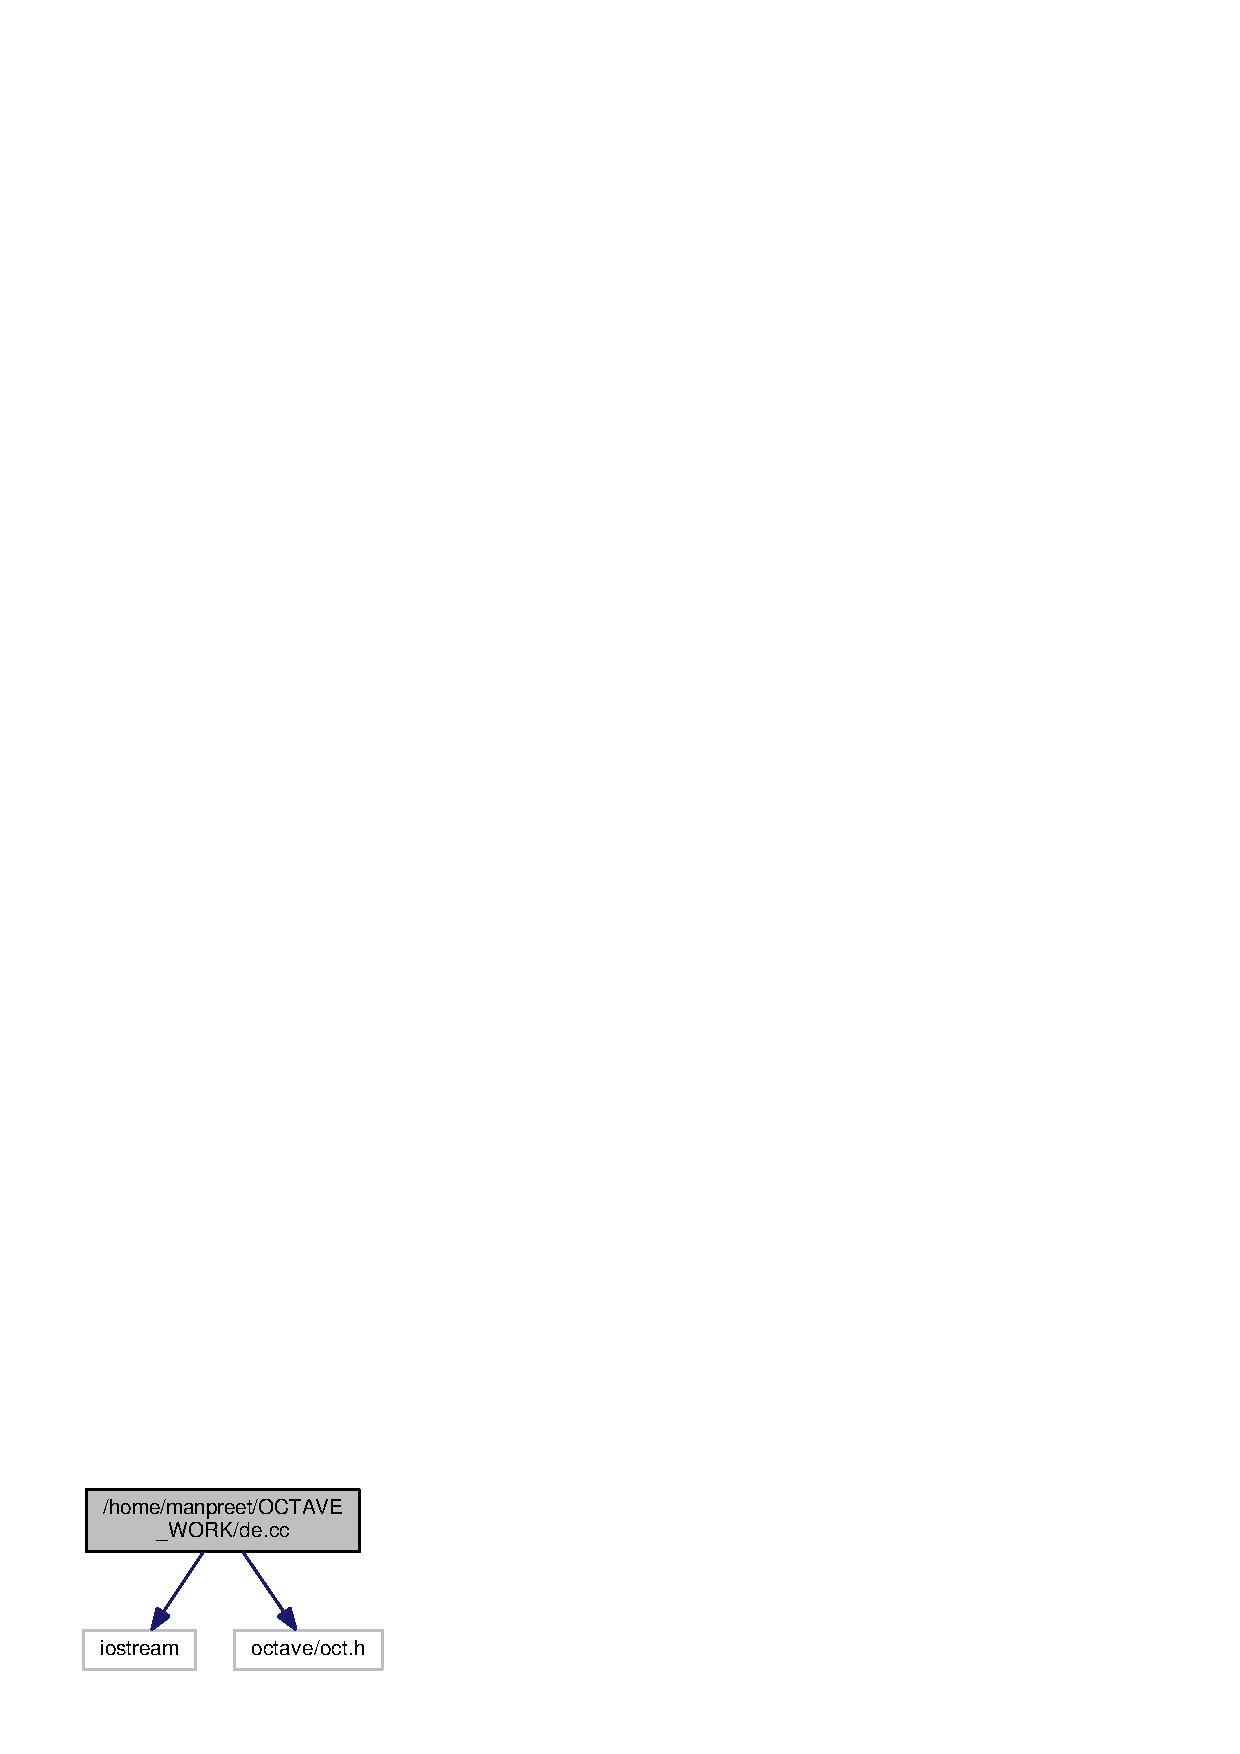
\includegraphics[width=187pt]{de_8cc__incl}
\end{center}
\end{figure}
\subsection*{Functions}
\begin{DoxyCompactItemize}
\item 
int {\bf main} ()
\end{DoxyCompactItemize}


\subsection{Function Documentation}
\index{de.\-cc@{de.\-cc}!main@{main}}
\index{main@{main}!de.cc@{de.\-cc}}
\subsubsection[{main}]{\setlength{\rightskip}{0pt plus 5cm}int main (
\begin{DoxyParamCaption}
{}
\end{DoxyParamCaption}
)}\label{de_8cc_ae66f6b31b5ad750f1fe042a706a4e3d4}


Definition at line 4 of file de.\-cc.


\begin{DoxyCode}
5 \{
6 
7 std::cout<<\textcolor{stringliteral}{" octave program \(\backslash\)n"};    \textcolor{comment}{//std is use for standard library.u can include using namespace std; in
       header. in this case dont usestd::}
8 \textcolor{keywordtype}{int} n=4;
9 std:: cout<<n<<\textcolor{stringliteral}{"\(\backslash\)n"};
10 
11 \}
\end{DoxyCode}

\section{/home/manpreet/\-O\-C\-T\-A\-V\-E\-\_\-\-W\-O\-R\-K/demo.m File Reference}
\label{demo_8m}\index{/home/manpreet/\-O\-C\-T\-A\-V\-E\-\_\-\-W\-O\-R\-K/demo.\-m@{/home/manpreet/\-O\-C\-T\-A\-V\-E\-\_\-\-W\-O\-R\-K/demo.\-m}}

\section{/home/manpreet/\-O\-C\-T\-A\-V\-E\-\_\-\-W\-O\-R\-K/democ++.cc File Reference}
\label{democ_09_09_8cc}\index{/home/manpreet/\-O\-C\-T\-A\-V\-E\-\_\-\-W\-O\-R\-K/democ++.\-cc@{/home/manpreet/\-O\-C\-T\-A\-V\-E\-\_\-\-W\-O\-R\-K/democ++.\-cc}}
{\ttfamily \#include $<$iostream$>$}\\*
Include dependency graph for democ++.cc\-:\nopagebreak
\begin{figure}[H]
\begin{center}
\leavevmode
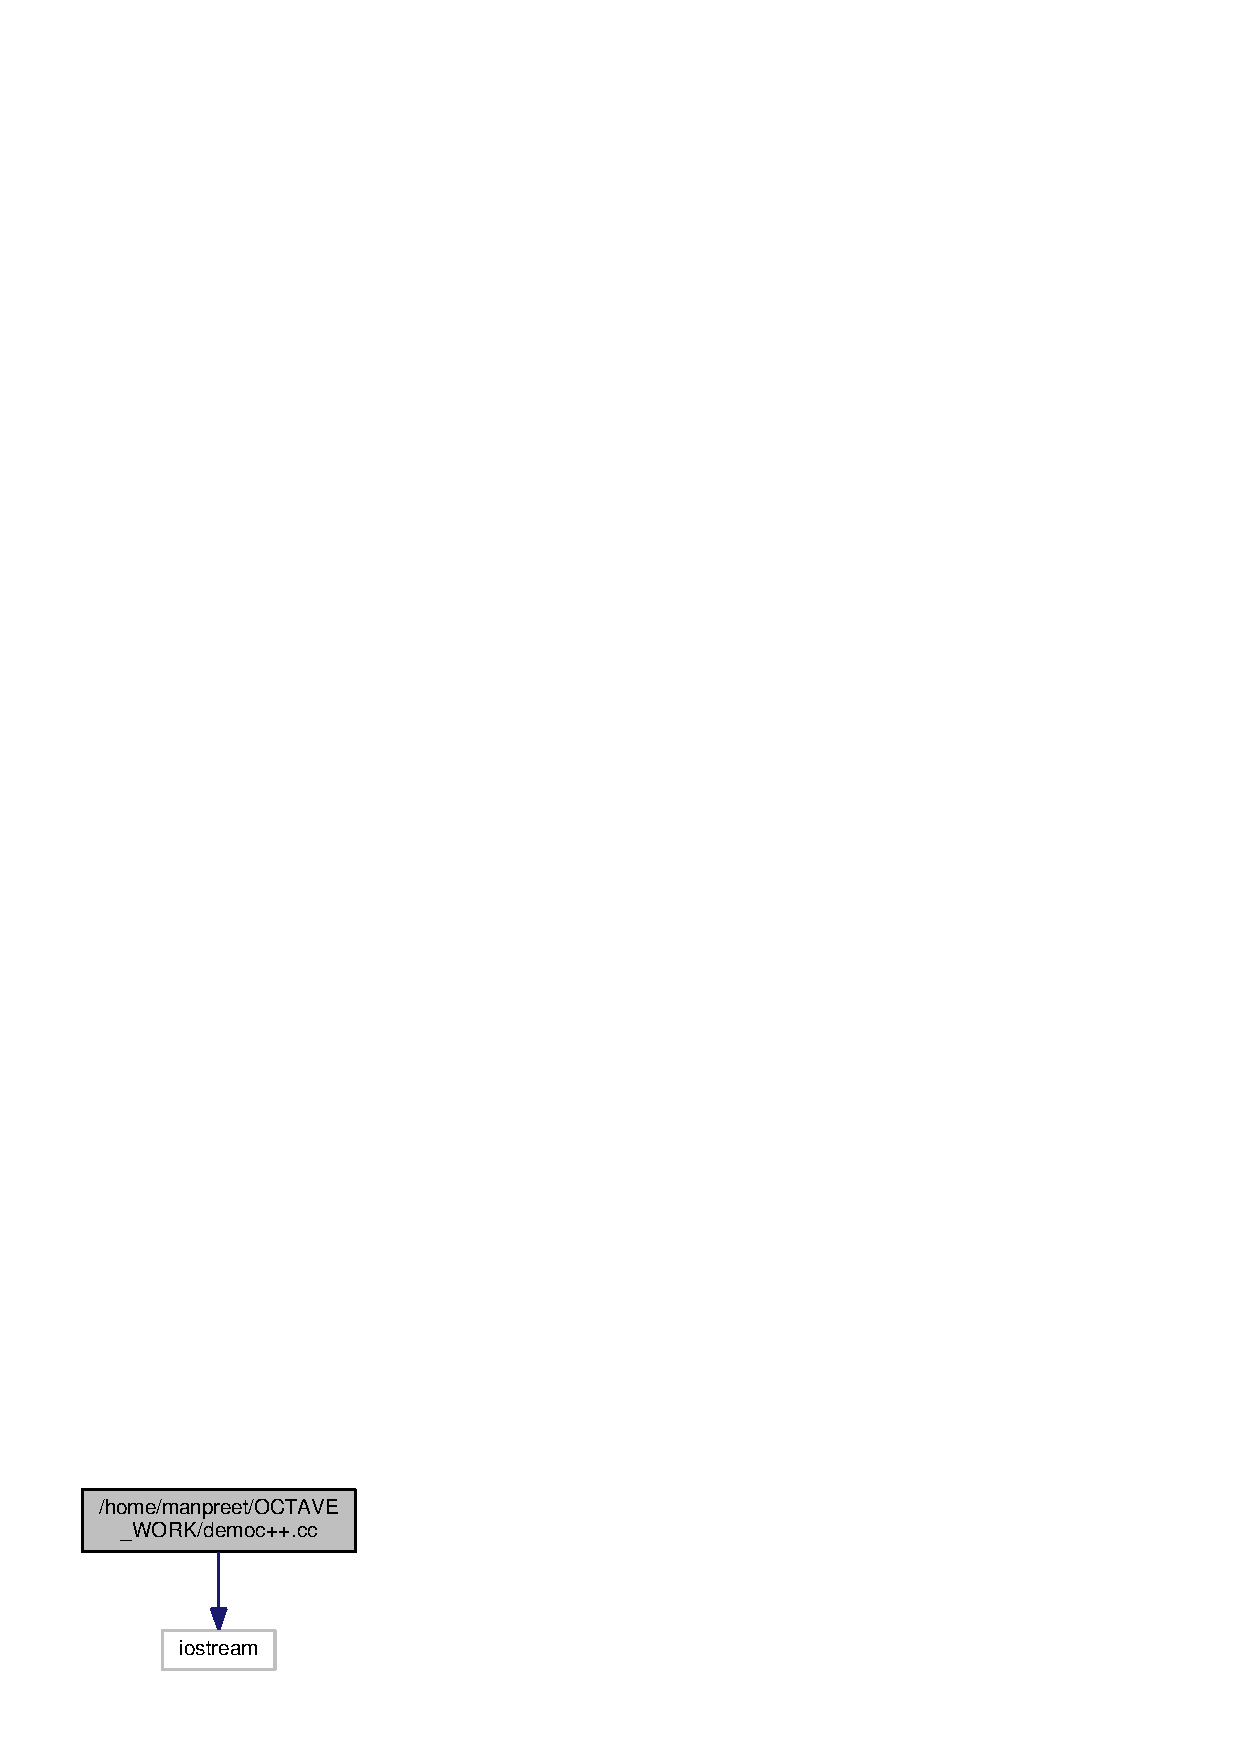
\includegraphics[width=174pt]{democ_09_09_8cc__incl}
\end{center}
\end{figure}
\subsection*{Functions}
\begin{DoxyCompactItemize}
\item 
int {\bf main} ()
\end{DoxyCompactItemize}


\subsection{Function Documentation}
\index{democ++.\-cc@{democ++.\-cc}!main@{main}}
\index{main@{main}!democ++.cc@{democ++.\-cc}}
\subsubsection[{main}]{\setlength{\rightskip}{0pt plus 5cm}int main (
\begin{DoxyParamCaption}
{}
\end{DoxyParamCaption}
)}\label{democ_09_09_8cc_ae66f6b31b5ad750f1fe042a706a4e3d4}


Definition at line 3 of file democ++.\-cc.



References i.


\begin{DoxyCode}
4 \{
5     \textcolor{keywordtype}{int} i=23;
6     \textcolor{comment}{// JUST ENTER ANY FLOAT VALUE LIKE 2.222}
7     cin>>i;
8     cin>>i;
9     cout<<i;
10 \}
\end{DoxyCode}

\section{/home/manpreet/\-O\-C\-T\-A\-V\-E\-\_\-\-W\-O\-R\-K/func.m File Reference}
\label{func_8m}\index{/home/manpreet/\-O\-C\-T\-A\-V\-E\-\_\-\-W\-O\-R\-K/func.\-m@{/home/manpreet/\-O\-C\-T\-A\-V\-E\-\_\-\-W\-O\-R\-K/func.\-m}}
\subsection*{Functions}
\begin{DoxyCompactItemize}
\item 
{\bf function} {\bf wakeup} ({\bf message}) printf(\char`\"{}\textbackslash{}a \%s \textbackslash{}n\char`\"{}
\end{DoxyCompactItemize}
\subsection*{Variables}
\begin{DoxyCompactItemize}
\item 
{\bf function} {\bf message}
\end{DoxyCompactItemize}


\subsection{Function Documentation}
\index{func.\-m@{func.\-m}!wakeup@{wakeup}}
\index{wakeup@{wakeup}!func.m@{func.\-m}}
\subsubsection[{wakeup}]{\setlength{\rightskip}{0pt plus 5cm}{\bf function} wakeup (
\begin{DoxyParamCaption}
\item[{{\bf message}}]{}
\end{DoxyParamCaption}
)}\label{func_8m_a9dcc41ecc4dccc4464aae33e30cfe53f}


\subsection{Variable Documentation}
\index{func.\-m@{func.\-m}!message@{message}}
\index{message@{message}!func.m@{func.\-m}}
\subsubsection[{message}]{\setlength{\rightskip}{0pt plus 5cm}{\bf function} message}\label{func_8m_a4859ee50f2aaabc934e6c09ada331dd5}


Definition at line 2 of file func.\-m.


\section{/home/manpreet/\-O\-C\-T\-A\-V\-E\-\_\-\-W\-O\-R\-K/func\-\_\-main.m File Reference}
\label{func__main_8m}\index{/home/manpreet/\-O\-C\-T\-A\-V\-E\-\_\-\-W\-O\-R\-K/func\-\_\-main.\-m@{/home/manpreet/\-O\-C\-T\-A\-V\-E\-\_\-\-W\-O\-R\-K/func\-\_\-main.\-m}}
\subsection*{Functions}
\begin{DoxyCompactItemize}
\item 
{\bf if} ({\bf storey\-\_\-i}$<$ Number\-\_\-of\-\_\-storeys) {\bf Stiffness\-\_\-matrix}({\bf storey\-\_\-i} = 1. + 15 $\ast$ time\-Prd
\item 
{\bf Stiffness\-\_\-matrix} ({\bf storey\-\_\-i}, {\bf storey\-\_\-i}+1)
\item 
{\bf Stiffness\-\_\-matrix} ({\bf storey\-\_\-i}+1, {\bf storey\-\_\-i})
\item 
{\bf if} ({\bf storey\-\_\-i} $>$1) {\bf Level\-\_\-floor}({\bf storey\-\_\-i}
\item 
end {\bf Modal\-\_\-participation\-\_\-factor} ({\bf index\-\_\-k}, 1)
\item 
{\bf Modal\-\_\-mass} ({\bf index\-\_\-k}, 1)
\item 
{\bf if} ({\bf Modes\-Contribution\-X} $>$ 90) break
\item 
endif end {\bf if} (Modes\-\_\-considered==0) Modes\-\_\-considered
\item 
{\bf A\-\_\-h} (index\-\_\-time, 1)
\item 
{\bf Peak\-\_\-shear\-\_\-force} ({\bf index\-\_\-i}, {\bf index\-\_\-j})
\item 
{\bf Storey\-\_\-shear\-\_\-force} ({\bf index\-\_\-i}, 2)
\item 
otherwise {\bf warning} ('Unexpected soil type')
\item 
{\bf elseif} (time\-Prd $>$ {\bf t3}) {\bf sag}
\item 
end end {\bf function} {\bf matrix\-Te\-X} ({\bf A}, fmt, align) disp(['\textbackslash{}section
\end{DoxyCompactItemize}
\subsection*{Variables}
\begin{DoxyCompactItemize}
\item 
{\bf clc} {\bf clear} load input mat {\bf function} {\bf Stiffness\-\_\-matrix}
\item 
{\bf storey\-\_\-i}
\item 
endif end end {\bf function} {\bf Level\-\_\-floor}
\item 
endif end end {\bf function} [Time\-\_\-period, Frequency, Time\-\_\-periods]
\item 
{\bf Omega} = sqrt(Omega\-\_\-square)
\item 
for {\bf index\-\_\-k}
\item 
{\bf sum\-\_\-\-W\-\_\-\-Phi2} = 0
\item 
for {\bf index\-\_\-i}
\item 
{\bf sum\-\_\-modal\-\_\-mass} = sum\-\_\-modal\-\_\-mass + {\bf Modal\-\_\-mass}({\bf index\-\_\-k},1)
\item 
end {\bf Modal\-\_\-contribution} = 100 / {\bf sum\-\_\-modal\-\_\-mass} $\ast$ {\bf Modal\-\_\-mass}
\item 
{\bf Modes\-Contribution\-X} = 0
\item 
{\bf Number\-\_\-of\-\_\-modes\-\_\-to\-\_\-be\-\_\-considered} = 0
\item 
end {\bf Peak\-\_\-shear\-\_\-force} = zeros(Number\-\_\-of\-\_\-storeys, Number\-\_\-of\-\_\-storeys,'double')
\item 
for {\bf index\-\_\-j}
\item 
{\bf index\-\_\-i} {\bf index\-\_\-j} {\bf index\-\_\-k} end \\*
end end end {\bf function} {\bf Storey\-\_\-shear\-\_\-force} = storey\-\_\-shear({\bf Peak\-\_\-shear\-\_\-force},Modes\-\_\-considered,Number\-\_\-of\-\_\-storeys) Storey\-\_\-shear\-\_\-force = zeros(Number\-\_\-of\-\_\-storeys, 3)
\item 
for {\bf i}
\item 
end Function to write Matrix {\bf t1} = 0
\item 
{\bf t2} = 0
\item 
{\bf t3} = 0
\item 
{\bf t4} = 0
\item 
{\bf eq3num} = 0
\item 
{\bf function} {\bf sag}
\end{DoxyCompactItemize}


\subsection{Function Documentation}
\index{func\-\_\-main.\-m@{func\-\_\-main.\-m}!A\-\_\-h@{A\-\_\-h}}
\index{A\-\_\-h@{A\-\_\-h}!func_main.m@{func\-\_\-main.\-m}}
\subsubsection[{A\-\_\-h}]{\setlength{\rightskip}{0pt plus 5cm}A\-\_\-h (
\begin{DoxyParamCaption}
\item[{index\-\_\-time}]{, }
\item[{1}]{}
\end{DoxyParamCaption}
)}\label{func__main_8m_aaf04dac8ecc9d475ba966025eba2915f}
\index{func\-\_\-main.\-m@{func\-\_\-main.\-m}!elseif@{elseif}}
\index{elseif@{elseif}!func_main.m@{func\-\_\-main.\-m}}
\subsubsection[{elseif}]{\setlength{\rightskip}{0pt plus 5cm}elseif (
\begin{DoxyParamCaption}
\item[{time\-Prd}]{, }
\item[{{\bf t3}}]{}
\end{DoxyParamCaption}
)}\label{func__main_8m_a0d135864d9bc0103cbd903c62d64b088}
\index{func\-\_\-main.\-m@{func\-\_\-main.\-m}!if@{if}}
\index{if@{if}!func_main.m@{func\-\_\-main.\-m}}
\subsubsection[{if}]{\setlength{\rightskip}{0pt plus 5cm}end if (
\begin{DoxyParamCaption}
{}
\end{DoxyParamCaption}
) = 1. + 15 $\ast$ time\-Prd}\label{func__main_8m_a07aafb5a4870a6777f2e28d7dc791b20}
\index{func\-\_\-main.\-m@{func\-\_\-main.\-m}!if@{if}}
\index{if@{if}!func_main.m@{func\-\_\-main.\-m}}
\subsubsection[{if}]{\setlength{\rightskip}{0pt plus 5cm}if (
\begin{DoxyParamCaption}
\item[{{\bf storey\-\_\-i}}]{, }
\item[{1}]{}
\end{DoxyParamCaption}
)}\label{func__main_8m_acae4743f53a057e86b2f94b495c656cb}
\index{func\-\_\-main.\-m@{func\-\_\-main.\-m}!if@{if}}
\index{if@{if}!func_main.m@{func\-\_\-main.\-m}}
\subsubsection[{if}]{\setlength{\rightskip}{0pt plus 5cm}if (
\begin{DoxyParamCaption}
\item[{{\bf Modes\-Contribution\-X}}]{, }
\item[{90}]{}
\end{DoxyParamCaption}
)}\label{func__main_8m_ae0824117b26ada50434e680632cec743}
\index{func\-\_\-main.\-m@{func\-\_\-main.\-m}!if@{if}}
\index{if@{if}!func_main.m@{func\-\_\-main.\-m}}
\subsubsection[{if}]{\setlength{\rightskip}{0pt plus 5cm}endif end if (
\begin{DoxyParamCaption}
\item[{Modes\-\_\-considered}]{ = {\ttfamily =0}}
\end{DoxyParamCaption}
)}\label{func__main_8m_a02b22951c30ac7239b551ac8b5c6d61b}
\index{func\-\_\-main.\-m@{func\-\_\-main.\-m}!matrix\-Te\-X@{matrix\-Te\-X}}
\index{matrix\-Te\-X@{matrix\-Te\-X}!func_main.m@{func\-\_\-main.\-m}}
\subsubsection[{matrix\-Te\-X}]{\setlength{\rightskip}{0pt plus 5cm}end end {\bf function} matrix\-Te\-X (
\begin{DoxyParamCaption}
\item[{{\bf A}}]{, }
\item[{fmt}]{, }
\item[{align}]{}
\end{DoxyParamCaption}
)}\label{func__main_8m_a8c0a4f44ca03289871d3743578e0412c}


Definition at line 187 of file func\-\_\-main.\-m.

\index{func\-\_\-main.\-m@{func\-\_\-main.\-m}!Modal\-\_\-mass@{Modal\-\_\-mass}}
\index{Modal\-\_\-mass@{Modal\-\_\-mass}!func_main.m@{func\-\_\-main.\-m}}
\subsubsection[{Modal\-\_\-mass}]{\setlength{\rightskip}{0pt plus 5cm}Modal\-\_\-mass (
\begin{DoxyParamCaption}
\item[{{\bf index\-\_\-k}}]{, }
\item[{1}]{}
\end{DoxyParamCaption}
)}\label{func__main_8m_ad609d920246c497257e51a2ccd326daa}
\index{func\-\_\-main.\-m@{func\-\_\-main.\-m}!Modal\-\_\-participation\-\_\-factor@{Modal\-\_\-participation\-\_\-factor}}
\index{Modal\-\_\-participation\-\_\-factor@{Modal\-\_\-participation\-\_\-factor}!func_main.m@{func\-\_\-main.\-m}}
\subsubsection[{Modal\-\_\-participation\-\_\-factor}]{\setlength{\rightskip}{0pt plus 5cm}end Modal\-\_\-participation\-\_\-factor (
\begin{DoxyParamCaption}
\item[{{\bf index\-\_\-k}}]{, }
\item[{1}]{}
\end{DoxyParamCaption}
)}\label{func__main_8m_a6a39cdc1dba79cf42ebb7ed3e4084d6d}
\index{func\-\_\-main.\-m@{func\-\_\-main.\-m}!Peak\-\_\-shear\-\_\-force@{Peak\-\_\-shear\-\_\-force}}
\index{Peak\-\_\-shear\-\_\-force@{Peak\-\_\-shear\-\_\-force}!func_main.m@{func\-\_\-main.\-m}}
\subsubsection[{Peak\-\_\-shear\-\_\-force}]{\setlength{\rightskip}{0pt plus 5cm}Peak\-\_\-shear\-\_\-force (
\begin{DoxyParamCaption}
\item[{{\bf index\-\_\-i}}]{, }
\item[{{\bf index\-\_\-j}}]{}
\end{DoxyParamCaption}
)}\label{func__main_8m_aa89dfab357a9a8af4c25d866bdcde2fd}
\index{func\-\_\-main.\-m@{func\-\_\-main.\-m}!Stiffness\-\_\-matrix@{Stiffness\-\_\-matrix}}
\index{Stiffness\-\_\-matrix@{Stiffness\-\_\-matrix}!func_main.m@{func\-\_\-main.\-m}}
\subsubsection[{Stiffness\-\_\-matrix}]{\setlength{\rightskip}{0pt plus 5cm}Stiffness\-\_\-matrix (
\begin{DoxyParamCaption}
\item[{{\bf storey\-\_\-i}}]{, }
\item[{{\bf storey\-\_\-i}+}]{1}
\end{DoxyParamCaption}
)}\label{func__main_8m_a26af3adbbfead21d609d8cbbcae4d612}
\index{func\-\_\-main.\-m@{func\-\_\-main.\-m}!Stiffness\-\_\-matrix@{Stiffness\-\_\-matrix}}
\index{Stiffness\-\_\-matrix@{Stiffness\-\_\-matrix}!func_main.m@{func\-\_\-main.\-m}}
\subsubsection[{Stiffness\-\_\-matrix}]{\setlength{\rightskip}{0pt plus 5cm}Stiffness\-\_\-matrix (
\begin{DoxyParamCaption}
\item[{{\bf storey\-\_\-i}+}]{1, }
\item[{{\bf storey\-\_\-i}}]{}
\end{DoxyParamCaption}
)}\label{func__main_8m_a5a8cf1f19d11fd73f873c351fddb387e}
\index{func\-\_\-main.\-m@{func\-\_\-main.\-m}!Storey\-\_\-shear\-\_\-force@{Storey\-\_\-shear\-\_\-force}}
\index{Storey\-\_\-shear\-\_\-force@{Storey\-\_\-shear\-\_\-force}!func_main.m@{func\-\_\-main.\-m}}
\subsubsection[{Storey\-\_\-shear\-\_\-force}]{\setlength{\rightskip}{0pt plus 5cm}Storey\-\_\-shear\-\_\-force (
\begin{DoxyParamCaption}
\item[{{\bf index\-\_\-i}}]{, }
\item[{2}]{}
\end{DoxyParamCaption}
)}\label{func__main_8m_a344dd6648691b1d2d2c3383d7bf04277}
\index{func\-\_\-main.\-m@{func\-\_\-main.\-m}!warning@{warning}}
\index{warning@{warning}!func_main.m@{func\-\_\-main.\-m}}
\subsubsection[{warning}]{\setlength{\rightskip}{0pt plus 5cm}otherwise warning (
\begin{DoxyParamCaption}
\item[{'Unexpected soil type'}]{}
\end{DoxyParamCaption}
)}\label{func__main_8m_ab503a94cad1959f242ec550d49261614}


\subsection{Variable Documentation}
\index{func\-\_\-main.\-m@{func\-\_\-main.\-m}!eq3num@{eq3num}}
\index{eq3num@{eq3num}!func_main.m@{func\-\_\-main.\-m}}
\subsubsection[{eq3num}]{\setlength{\rightskip}{0pt plus 5cm}eq3num = 0}\label{func__main_8m_a8ecbd124ddcdab7fc367443a82b241af}


Definition at line 162 of file func\-\_\-main.\-m.

\index{func\-\_\-main.\-m@{func\-\_\-main.\-m}!function@{function}}
\index{function@{function}!func_main.m@{func\-\_\-main.\-m}}
\subsubsection[{function}]{\setlength{\rightskip}{0pt plus 5cm}end end function}\label{func__main_8m_a3b7d315fa6e146442de88ccb3f470ea7}
{\bfseries Initial value\-:}
\begin{DoxyCode}
= eigenomega(Stiffness_matrix, Mass,Number\_of\_storeys)
[Eigen\_vector, Omega\_square] = eig(Stiffness_matrix, Mass)
\end{DoxyCode}


Definition at line 45 of file func\-\_\-main.\-m.

\index{func\-\_\-main.\-m@{func\-\_\-main.\-m}!i@{i}}
\index{i@{i}!func_main.m@{func\-\_\-main.\-m}}
\subsubsection[{i}]{\setlength{\rightskip}{0pt plus 5cm}for i}\label{func__main_8m_a6f6ccfcf58b31cb6412107d9d5281426}
{\bfseries Initial value\-:}
\begin{DoxyCode}
= 1:Soil\_type
 Type_of_soil = strcat(Type_of_soil, \textcolor{charliteral}{'I'})
\end{DoxyCode}


Definition at line 155 of file func\-\_\-main.\-m.

\index{func\-\_\-main.\-m@{func\-\_\-main.\-m}!index\-\_\-i@{index\-\_\-i}}
\index{index\-\_\-i@{index\-\_\-i}!func_main.m@{func\-\_\-main.\-m}}
\subsubsection[{index\-\_\-i}]{\setlength{\rightskip}{0pt plus 5cm}for index\-\_\-i}\label{func__main_8m_ac6e21a32e1cf6d0626600bb610d05c93}
{\bfseries Initial value\-:}
\begin{DoxyCode}
= 1 : Number\_of\_storeys
                                sum\_W\_Phi = sum\_W\_Phi + Mass(index_i, index_i) * ...
                                Eigen\_vector(index_i, index_k)
\end{DoxyCode}


Definition at line 65 of file func\-\_\-main.\-m.

\index{func\-\_\-main.\-m@{func\-\_\-main.\-m}!index\-\_\-j@{index\-\_\-j}}
\index{index\-\_\-j@{index\-\_\-j}!func_main.m@{func\-\_\-main.\-m}}
\subsubsection[{index\-\_\-j}]{\setlength{\rightskip}{0pt plus 5cm}for index\-\_\-j}\label{func__main_8m_a9d105c6932d303e9e7a82b49e9bc876a}
{\bfseries Initial value\-:}
\begin{DoxyCode}
= 1:Number\_of\_storeys
                \textcolor{keywordflow}{for} index_i = 1:Number\_of\_storeys
                        \textcolor{keywordflow}{for} index_k = 1:Number\_of\_storeys - index_i +1
                        % index\_m = index_k + index_i -1
\end{DoxyCode}


Definition at line 111 of file func\-\_\-main.\-m.

\index{func\-\_\-main.\-m@{func\-\_\-main.\-m}!index\-\_\-k@{index\-\_\-k}}
\index{index\-\_\-k@{index\-\_\-k}!func_main.m@{func\-\_\-main.\-m}}
\subsubsection[{index\-\_\-k}]{\setlength{\rightskip}{0pt plus 5cm}for index\-\_\-k}\label{func__main_8m_aeb7138595dee788b60a4aab95ea30ead}
{\bfseries Initial value\-:}
\begin{DoxyCode}
= 1 : Number\_of\_storeys
                sum\_W\_Phi = 0
\end{DoxyCode}


Definition at line 62 of file func\-\_\-main.\-m.

\index{func\-\_\-main.\-m@{func\-\_\-main.\-m}!Level\-\_\-floor@{Level\-\_\-floor}}
\index{Level\-\_\-floor@{Level\-\_\-floor}!func_main.m@{func\-\_\-main.\-m}}
\subsubsection[{Level\-\_\-floor}]{\setlength{\rightskip}{0pt plus 5cm}endif end end {\bf function} Level\-\_\-floor}\label{func__main_8m_afbcb7c65e7756ba8ad0c8011e8b9ec84}
{\bfseries Initial value\-:}
\begin{DoxyCode}
=levelf(Height\_storey)
        Number\_of\_storeys=4
\end{DoxyCode}


Definition at line 32 of file func\-\_\-main.\-m.

\index{func\-\_\-main.\-m@{func\-\_\-main.\-m}!Modal\-\_\-contribution@{Modal\-\_\-contribution}}
\index{Modal\-\_\-contribution@{Modal\-\_\-contribution}!func_main.m@{func\-\_\-main.\-m}}
\subsubsection[{Modal\-\_\-contribution}]{\setlength{\rightskip}{0pt plus 5cm}end Modal\-\_\-contribution = 100 / {\bf sum\-\_\-modal\-\_\-mass} $\ast$ {\bf Modal\-\_\-mass}}\label{func__main_8m_afc15fafadb4f9b24ca3f82f6b72bafcf}


Definition at line 76 of file func\-\_\-main.\-m.

\index{func\-\_\-main.\-m@{func\-\_\-main.\-m}!Modes\-Contribution\-X@{Modes\-Contribution\-X}}
\index{Modes\-Contribution\-X@{Modes\-Contribution\-X}!func_main.m@{func\-\_\-main.\-m}}
\subsubsection[{Modes\-Contribution\-X}]{\setlength{\rightskip}{0pt plus 5cm}Modes\-Contribution\-X = 0}\label{func__main_8m_a55f0e7d483cc95c31ab81c9bdcbed944}


Definition at line 78 of file func\-\_\-main.\-m.

\index{func\-\_\-main.\-m@{func\-\_\-main.\-m}!Number\-\_\-of\-\_\-modes\-\_\-to\-\_\-be\-\_\-considered@{Number\-\_\-of\-\_\-modes\-\_\-to\-\_\-be\-\_\-considered}}
\index{Number\-\_\-of\-\_\-modes\-\_\-to\-\_\-be\-\_\-considered@{Number\-\_\-of\-\_\-modes\-\_\-to\-\_\-be\-\_\-considered}!func_main.m@{func\-\_\-main.\-m}}
\subsubsection[{Number\-\_\-of\-\_\-modes\-\_\-to\-\_\-be\-\_\-considered}]{\setlength{\rightskip}{0pt plus 5cm}for Number\-\_\-of\-\_\-modes\-\_\-to\-\_\-be\-\_\-considered = 0}\label{func__main_8m_a1034ee45b0411e5b452175e522e6e87a}


Definition at line 79 of file func\-\_\-main.\-m.

\index{func\-\_\-main.\-m@{func\-\_\-main.\-m}!Omega@{Omega}}
\index{Omega@{Omega}!func_main.m@{func\-\_\-main.\-m}}
\subsubsection[{Omega}]{\setlength{\rightskip}{0pt plus 5cm}Omega = sqrt(Omega\-\_\-square)}\label{func__main_8m_abd44e0f647c914787c461677b6933451}


Definition at line 47 of file func\-\_\-main.\-m.

\index{func\-\_\-main.\-m@{func\-\_\-main.\-m}!Peak\-\_\-shear\-\_\-force@{Peak\-\_\-shear\-\_\-force}}
\index{Peak\-\_\-shear\-\_\-force@{Peak\-\_\-shear\-\_\-force}!func_main.m@{func\-\_\-main.\-m}}
\subsubsection[{Peak\-\_\-shear\-\_\-force}]{\setlength{\rightskip}{0pt plus 5cm}end Peak\-\_\-shear\-\_\-force = zeros(Number\-\_\-of\-\_\-storeys, Number\-\_\-of\-\_\-storeys,'double')}\label{func__main_8m_a5bf27342fe06cf8dc956564530a388ea}


Definition at line 110 of file func\-\_\-main.\-m.

\index{func\-\_\-main.\-m@{func\-\_\-main.\-m}!sag@{sag}}
\index{sag@{sag}!func_main.m@{func\-\_\-main.\-m}}
\subsubsection[{sag}]{\setlength{\rightskip}{0pt plus 5cm}else sag}\label{func__main_8m_aac9abc95cd2ddc27fa84fb4440b62888}
{\bfseries Initial value\-:}
\begin{DoxyCode}
= funSaog(soilType, timePrd)
    t2=0.10
\end{DoxyCode}


Definition at line 165 of file func\-\_\-main.\-m.

\index{func\-\_\-main.\-m@{func\-\_\-main.\-m}!Stiffness\-\_\-matrix@{Stiffness\-\_\-matrix}}
\index{Stiffness\-\_\-matrix@{Stiffness\-\_\-matrix}!func_main.m@{func\-\_\-main.\-m}}
\subsubsection[{Stiffness\-\_\-matrix}]{\setlength{\rightskip}{0pt plus 5cm}{\bf clc} {\bf clear} load input mat {\bf function} Stiffness\-\_\-matrix}\label{func__main_8m_a70c56f90084642dd078d3a85e443f00f}
{\bfseries Initial value\-:}
\begin{DoxyCode}
=stif(Stiffness\_storey,Number\_of\_storeys)



                for  storey_i = 1:Number\_of\_storeys

                        Stiffness_matrix(storey_i, storey\_i) = ...
                        Stiffness\_storey(storey\_i)
\end{DoxyCode}


Definition at line 10 of file func\-\_\-main.\-m.

\index{func\-\_\-main.\-m@{func\-\_\-main.\-m}!storey\-\_\-i@{storey\-\_\-i}}
\index{storey\-\_\-i@{storey\-\_\-i}!func_main.m@{func\-\_\-main.\-m}}
\subsubsection[{storey\-\_\-i}]{\setlength{\rightskip}{0pt plus 5cm}end for storey\-\_\-i}\label{func__main_8m_a6f92001683fd75ef72b08797cda8d28e}
{\bfseries Initial value\-:}
\begin{DoxyCode}
= ...
                                Stiffness_matrix(storey_i, storey_i) + ...
                                Stiffness\_storey(storey_i + 1)
\end{DoxyCode}


Definition at line 20 of file func\-\_\-main.\-m.

\index{func\-\_\-main.\-m@{func\-\_\-main.\-m}!Storey\-\_\-shear\-\_\-force@{Storey\-\_\-shear\-\_\-force}}
\index{Storey\-\_\-shear\-\_\-force@{Storey\-\_\-shear\-\_\-force}!func_main.m@{func\-\_\-main.\-m}}
\subsubsection[{Storey\-\_\-shear\-\_\-force}]{\setlength{\rightskip}{0pt plus 5cm}end Storey\-\_\-shear\-\_\-force = storey\-\_\-shear({\bf Peak\-\_\-shear\-\_\-force},Modes\-\_\-considered,Number\-\_\-of\-\_\-storeys) Storey\-\_\-shear\-\_\-force = zeros(Number\-\_\-of\-\_\-storeys, 3)}\label{func__main_8m_a134fef5d3009a6da1f3b70334b85bc3e}


Definition at line 127 of file func\-\_\-main.\-m.

\index{func\-\_\-main.\-m@{func\-\_\-main.\-m}!sum\-\_\-modal\-\_\-mass@{sum\-\_\-modal\-\_\-mass}}
\index{sum\-\_\-modal\-\_\-mass@{sum\-\_\-modal\-\_\-mass}!func_main.m@{func\-\_\-main.\-m}}
\subsubsection[{sum\-\_\-modal\-\_\-mass}]{\setlength{\rightskip}{0pt plus 5cm}sum\-\_\-modal\-\_\-mass = sum\-\_\-modal\-\_\-mass + {\bf Modal\-\_\-mass}({\bf index\-\_\-k},1)}\label{func__main_8m_afe41102d21582a0644f2bb7795f858dd}


Definition at line 73 of file func\-\_\-main.\-m.

\index{func\-\_\-main.\-m@{func\-\_\-main.\-m}!sum\-\_\-\-W\-\_\-\-Phi2@{sum\-\_\-\-W\-\_\-\-Phi2}}
\index{sum\-\_\-\-W\-\_\-\-Phi2@{sum\-\_\-\-W\-\_\-\-Phi2}!func_main.m@{func\-\_\-main.\-m}}
\subsubsection[{sum\-\_\-\-W\-\_\-\-Phi2}]{\setlength{\rightskip}{0pt plus 5cm}sum\-\_\-\-W\-\_\-\-Phi2 = 0}\label{func__main_8m_ab396194af7ea5f2a640654cd83b07e1f}


Definition at line 64 of file func\-\_\-main.\-m.

\index{func\-\_\-main.\-m@{func\-\_\-main.\-m}!t1@{t1}}
\index{t1@{t1}!func_main.m@{func\-\_\-main.\-m}}
\subsubsection[{t1}]{\setlength{\rightskip}{0pt plus 5cm}t1 = 0}\label{func__main_8m_a469994e78f66a44815c015b7f4b8b2f8}


Definition at line 161 of file func\-\_\-main.\-m.

\index{func\-\_\-main.\-m@{func\-\_\-main.\-m}!t2@{t2}}
\index{t2@{t2}!func_main.m@{func\-\_\-main.\-m}}
\subsubsection[{t2}]{\setlength{\rightskip}{0pt plus 5cm}t2 = 0}\label{func__main_8m_a24aeadb733f27244ec14e4cba82eeee9}


Definition at line 161 of file func\-\_\-main.\-m.

\index{func\-\_\-main.\-m@{func\-\_\-main.\-m}!t3@{t3}}
\index{t3@{t3}!func_main.m@{func\-\_\-main.\-m}}
\subsubsection[{t3}]{\setlength{\rightskip}{0pt plus 5cm}case I\-I\-I t3 = 0}\label{func__main_8m_a80d62394ff82e3ae283e9113bca340a2}


Definition at line 161 of file func\-\_\-main.\-m.

\index{func\-\_\-main.\-m@{func\-\_\-main.\-m}!t4@{t4}}
\index{t4@{t4}!func_main.m@{func\-\_\-main.\-m}}
\subsubsection[{t4}]{\setlength{\rightskip}{0pt plus 5cm}t4 = 0}\label{func__main_8m_ae95ab11d59379638967673bd74654b2a}


Definition at line 161 of file func\-\_\-main.\-m.


\section{/home/manpreet/\-O\-C\-T\-A\-V\-E\-\_\-\-W\-O\-R\-K/imageproces.m File Reference}
\label{imageproces_8m}\index{/home/manpreet/\-O\-C\-T\-A\-V\-E\-\_\-\-W\-O\-R\-K/imageproces.\-m@{/home/manpreet/\-O\-C\-T\-A\-V\-E\-\_\-\-W\-O\-R\-K/imageproces.\-m}}

\section{/home/manpreet/\-O\-C\-T\-A\-V\-E\-\_\-\-W\-O\-R\-K/imgp.cc File Reference}
\label{imgp_8cc}\index{/home/manpreet/\-O\-C\-T\-A\-V\-E\-\_\-\-W\-O\-R\-K/imgp.\-cc@{/home/manpreet/\-O\-C\-T\-A\-V\-E\-\_\-\-W\-O\-R\-K/imgp.\-cc}}
{\ttfamily \#include $<$iostream$>$}\\*
{\ttfamily \#include $<$octave/oct.\-h$>$}\\*
{\ttfamily \#include \char`\"{}graphics.\-h\char`\"{}}\\*
Include dependency graph for imgp.\-cc\-:\nopagebreak
\begin{figure}[H]
\begin{center}
\leavevmode
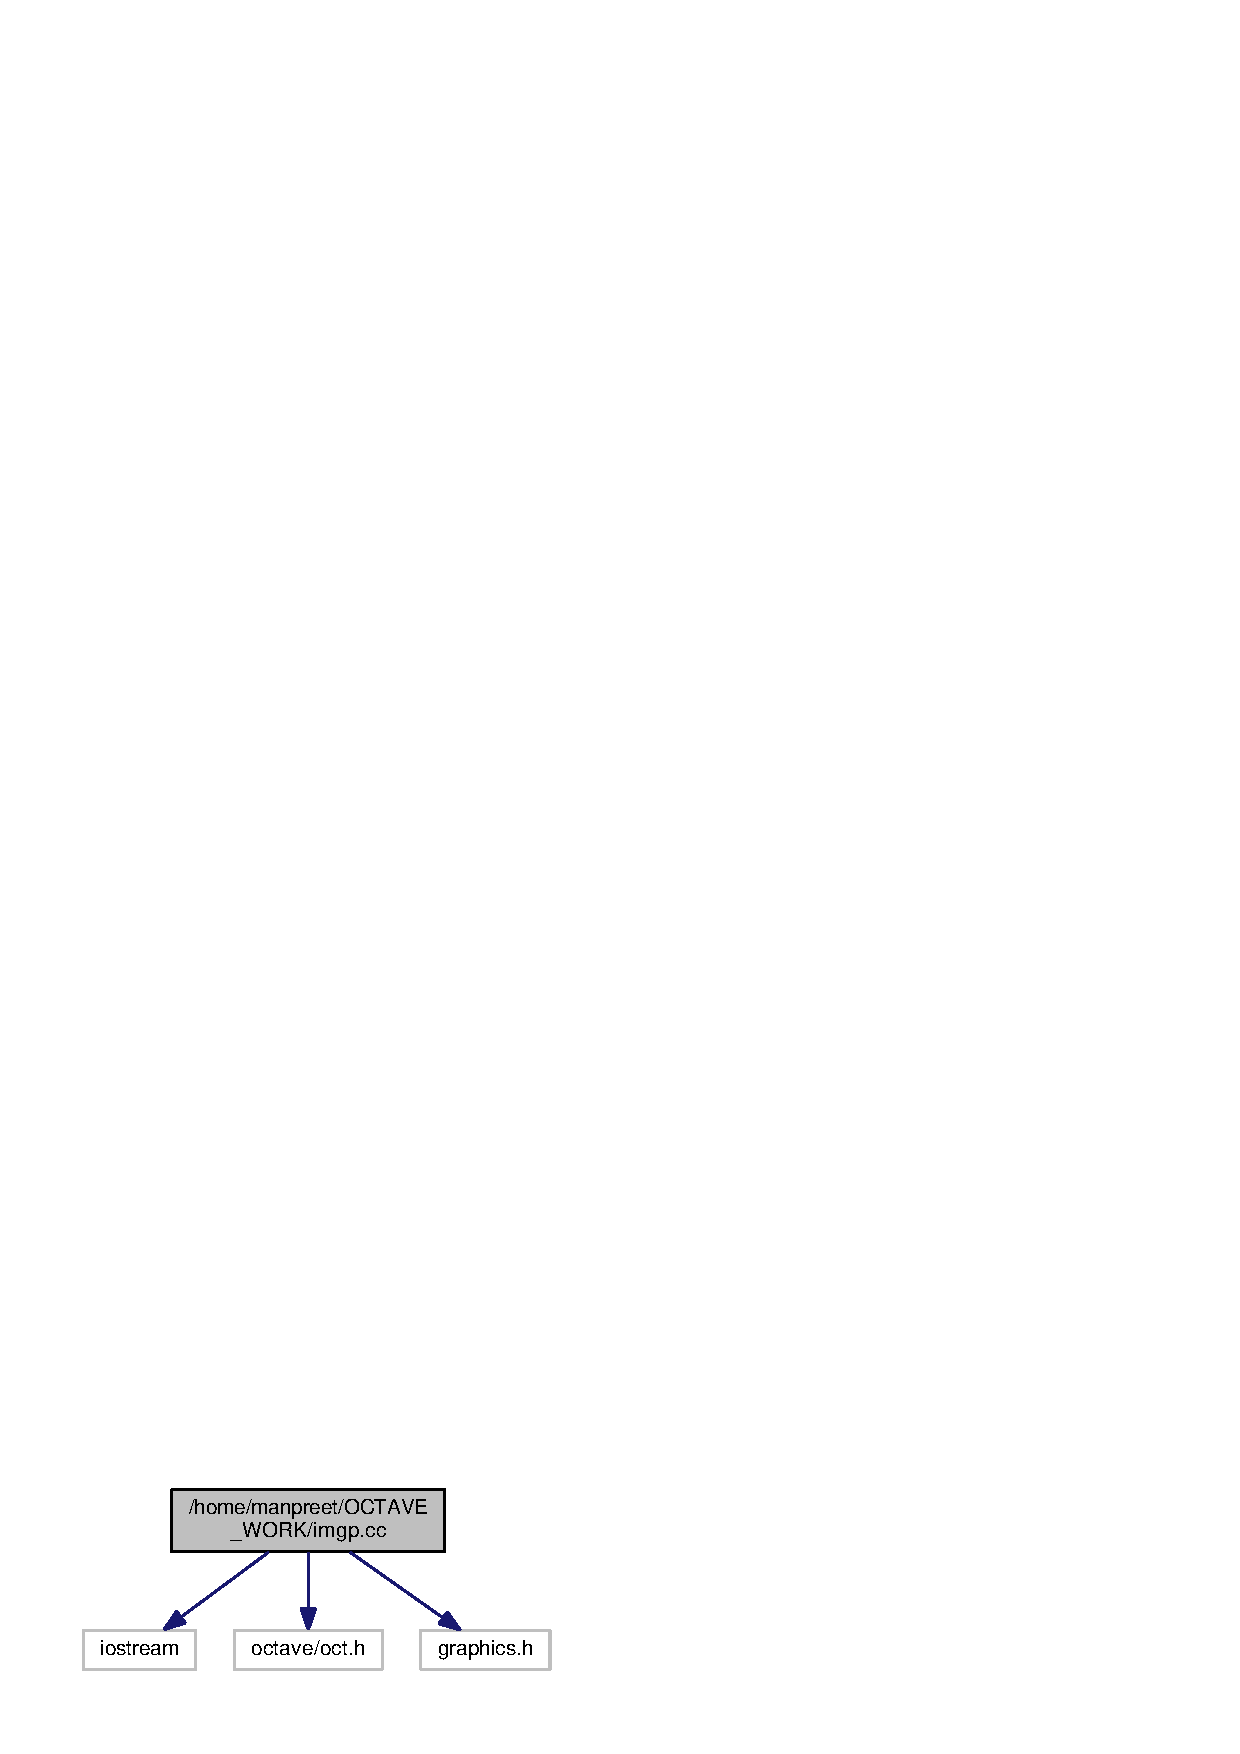
\includegraphics[width=268pt]{imgp_8cc__incl}
\end{center}
\end{figure}
\subsection*{Functions}
\begin{DoxyCompactItemize}
\item 
int {\bf main} ()
\end{DoxyCompactItemize}


\subsection{Function Documentation}
\index{imgp.\-cc@{imgp.\-cc}!main@{main}}
\index{main@{main}!imgp.cc@{imgp.\-cc}}
\subsubsection[{main}]{\setlength{\rightskip}{0pt plus 5cm}int main (
\begin{DoxyParamCaption}
{}
\end{DoxyParamCaption}
)}\label{imgp_8cc_ae66f6b31b5ad750f1fe042a706a4e3d4}


Definition at line 6 of file imgp.\-cc.


\begin{DoxyCode}
7 \{
8   Matrix  img;
9   img=img.imread(\textcolor{stringliteral}{"/home/manpreet/Desktop/nature1.jpg"});
10   imshow(img);
11   \textcolor{keywordflow}{return} 0;
12 \}
\end{DoxyCode}

\section{/home/manpreet/\-O\-C\-T\-A\-V\-E\-\_\-\-W\-O\-R\-K/inputfile.m File Reference}
\label{inputfile_8m}\index{/home/manpreet/\-O\-C\-T\-A\-V\-E\-\_\-\-W\-O\-R\-K/inputfile.\-m@{/home/manpreet/\-O\-C\-T\-A\-V\-E\-\_\-\-W\-O\-R\-K/inputfile.\-m}}
\subsection*{Functions}
\begin{DoxyCompactItemize}
\item 
{\bf fprintf} ({\bf file2}, '\%{\bf i}\%i\textbackslash{}n', {\bf A})
\item 
{\bf fclose} ({\bf file2})
\end{DoxyCompactItemize}
\subsection*{Variables}
\begin{DoxyCompactItemize}
\item 
{\bf clear}
\item 
{\bf clc}
\item 
{\bf A} =[1 2
\item 
{\bf file2} =fopen('matrix.\-txt', 'w')
\end{DoxyCompactItemize}


\subsection{Function Documentation}
\index{inputfile.\-m@{inputfile.\-m}!fclose@{fclose}}
\index{fclose@{fclose}!inputfile.m@{inputfile.\-m}}
\subsubsection[{fclose}]{\setlength{\rightskip}{0pt plus 5cm}fclose (
\begin{DoxyParamCaption}
\item[{{\bf file2}}]{}
\end{DoxyParamCaption}
)}\label{inputfile_8m_a09cdb01fc6e1c79f3adfbca5a482c967}
\index{inputfile.\-m@{inputfile.\-m}!fprintf@{fprintf}}
\index{fprintf@{fprintf}!inputfile.m@{inputfile.\-m}}
\subsubsection[{fprintf}]{\setlength{\rightskip}{0pt plus 5cm}fprintf (
\begin{DoxyParamCaption}
\item[{{\bf file2}}]{, }
\item[{'\%{\bf i}\%i\textbackslash{}n'}]{, }
\item[{{\bf A}}]{}
\end{DoxyParamCaption}
)}\label{inputfile_8m_ad88b870bbdc1da78fb2868ef445194bd}


\subsection{Variable Documentation}
\index{inputfile.\-m@{inputfile.\-m}!A@{A}}
\index{A@{A}!inputfile.m@{inputfile.\-m}}
\subsubsection[{A}]{\setlength{\rightskip}{0pt plus 5cm}A =[1 2}\label{inputfile_8m_a3b98e2dffc6cb06a89dcb0d5c60a0206}


Definition at line 3 of file inputfile.\-m.

\index{inputfile.\-m@{inputfile.\-m}!clc@{clc}}
\index{clc@{clc}!inputfile.m@{inputfile.\-m}}
\subsubsection[{clc}]{\setlength{\rightskip}{0pt plus 5cm}clc}\label{inputfile_8m_a3f3d3b13a15c726d6aa03db3dd0d6377}


Definition at line 2 of file inputfile.\-m.

\index{inputfile.\-m@{inputfile.\-m}!clear@{clear}}
\index{clear@{clear}!inputfile.m@{inputfile.\-m}}
\subsubsection[{clear}]{\setlength{\rightskip}{0pt plus 5cm}clear}\label{inputfile_8m_aebfdce4f6cc7241ba38924f77a12e7cf}


Definition at line 2 of file inputfile.\-m.

\index{inputfile.\-m@{inputfile.\-m}!file2@{file2}}
\index{file2@{file2}!inputfile.m@{inputfile.\-m}}
\subsubsection[{file2}]{\setlength{\rightskip}{0pt plus 5cm}file2 =fopen('matrix.\-txt', 'w')}\label{inputfile_8m_a1858d01a8d84806c9998f8ec81e9b774}


Definition at line 4 of file inputfile.\-m.


\section{/home/manpreet/\-O\-C\-T\-A\-V\-E\-\_\-\-W\-O\-R\-K/main.m File Reference}
\label{main_8m}\index{/home/manpreet/\-O\-C\-T\-A\-V\-E\-\_\-\-W\-O\-R\-K/main.\-m@{/home/manpreet/\-O\-C\-T\-A\-V\-E\-\_\-\-W\-O\-R\-K/main.\-m}}
\subsection*{Variables}
\begin{DoxyCompactItemize}
\item 
{\bf B} =[1 2
\end{DoxyCompactItemize}


\subsection{Variable Documentation}
\index{main.\-m@{main.\-m}!B@{B}}
\index{B@{B}!main.m@{main.\-m}}
\subsubsection[{B}]{\setlength{\rightskip}{0pt plus 5cm}B =[1 2}\label{main_8m_a9d3d9048db16a7eee539e93e3618cbe7}


Definition at line 1 of file main.\-m.


\section{/home/manpreet/\-O\-C\-T\-A\-V\-E\-\_\-\-W\-O\-R\-K/maincivil.m File Reference}
\label{maincivil_8m}\index{/home/manpreet/\-O\-C\-T\-A\-V\-E\-\_\-\-W\-O\-R\-K/maincivil.\-m@{/home/manpreet/\-O\-C\-T\-A\-V\-E\-\_\-\-W\-O\-R\-K/maincivil.\-m}}
\subsection*{Functions}
\begin{DoxyCompactItemize}
\item 
{\bf fdisp} ({\bf fid},\char`\"{}3/8 is \char`\"{})
\item 
{\bf fdisp} ({\bf fid}, 3/8)
\item 
{\bf fdisp} (\char`\"{}nums1.\-txt\char`\"{}, x)
\item 
{\bf fdisp} ({\bf fid}, val)
\item 
{\bf fclose} ({\bf fid})
\end{DoxyCompactItemize}
\subsection*{Variables}
\begin{DoxyCompactItemize}
\item 
{\bf x} =12345
\item 
{\bf fid} = fopen (\char`\"{}nums1.\-txt\char`\"{}, 'w')
\end{DoxyCompactItemize}


\subsection{Function Documentation}
\index{maincivil.\-m@{maincivil.\-m}!fclose@{fclose}}
\index{fclose@{fclose}!maincivil.m@{maincivil.\-m}}
\subsubsection[{fclose}]{\setlength{\rightskip}{0pt plus 5cm}fclose (
\begin{DoxyParamCaption}
\item[{{\bf fid}}]{}
\end{DoxyParamCaption}
)}\label{maincivil_8m_a5e769bbbabcaddc548203741c7100228}
\index{maincivil.\-m@{maincivil.\-m}!fdisp@{fdisp}}
\index{fdisp@{fdisp}!maincivil.m@{maincivil.\-m}}
\subsubsection[{fdisp}]{\setlength{\rightskip}{0pt plus 5cm}fdisp (
\begin{DoxyParamCaption}
\item[{{\bf fid}}]{, }
\item[{\char`\"{}3/8 is \char`\"{}}]{}
\end{DoxyParamCaption}
)}\label{maincivil_8m_af96c907665d1e7ae8e19366548b44814}
\index{maincivil.\-m@{maincivil.\-m}!fdisp@{fdisp}}
\index{fdisp@{fdisp}!maincivil.m@{maincivil.\-m}}
\subsubsection[{fdisp}]{\setlength{\rightskip}{0pt plus 5cm}fdisp (
\begin{DoxyParamCaption}
\item[{{\bf fid}}]{, }
\item[{3/}]{8}
\end{DoxyParamCaption}
)}\label{maincivil_8m_ab10dd89653b04a703d7a8edfa9b83385}
\index{maincivil.\-m@{maincivil.\-m}!fdisp@{fdisp}}
\index{fdisp@{fdisp}!maincivil.m@{maincivil.\-m}}
\subsubsection[{fdisp}]{\setlength{\rightskip}{0pt plus 5cm}fdisp (
\begin{DoxyParamCaption}
\item[{\char`\"{}nums1.\-txt\char`\"{}}]{, }
\item[{{\bf x}}]{}
\end{DoxyParamCaption}
)}\label{maincivil_8m_a6c6ac9157dc5b680621646feb6565925}
\index{maincivil.\-m@{maincivil.\-m}!fdisp@{fdisp}}
\index{fdisp@{fdisp}!maincivil.m@{maincivil.\-m}}
\subsubsection[{fdisp}]{\setlength{\rightskip}{0pt plus 5cm}fdisp (
\begin{DoxyParamCaption}
\item[{{\bf fid}}]{, }
\item[{val}]{}
\end{DoxyParamCaption}
)}\label{maincivil_8m_a45dd6fefa26134447e17daf8fc78418c}


\subsection{Variable Documentation}
\index{maincivil.\-m@{maincivil.\-m}!fid@{fid}}
\index{fid@{fid}!maincivil.m@{maincivil.\-m}}
\subsubsection[{fid}]{\setlength{\rightskip}{0pt plus 5cm}fid = fopen (\char`\"{}nums1.\-txt\char`\"{}, 'w')}\label{maincivil_8m_ae9011d40c6f13e68e6f07156e0da7c5d}


Definition at line 8 of file maincivil.\-m.

\index{maincivil.\-m@{maincivil.\-m}!x@{x}}
\index{x@{x}!maincivil.m@{maincivil.\-m}}
\subsubsection[{x}]{\setlength{\rightskip}{0pt plus 5cm}x =12345}\label{maincivil_8m_a9336ebf25087d91c818ee6e9ec29f8c1}


Definition at line 7 of file maincivil.\-m.


\section{/home/manpreet/\-O\-C\-T\-A\-V\-E\-\_\-\-W\-O\-R\-K/octcgi.cc File Reference}
\label{octcgi_8cc}\index{/home/manpreet/\-O\-C\-T\-A\-V\-E\-\_\-\-W\-O\-R\-K/octcgi.\-cc@{/home/manpreet/\-O\-C\-T\-A\-V\-E\-\_\-\-W\-O\-R\-K/octcgi.\-cc}}
{\ttfamily \#include $<$iostream$>$}\\*
{\ttfamily \#include $<$octave/oct.\-h$>$}\\*
Include dependency graph for octcgi.\-cc\-:\nopagebreak
\begin{figure}[H]
\begin{center}
\leavevmode
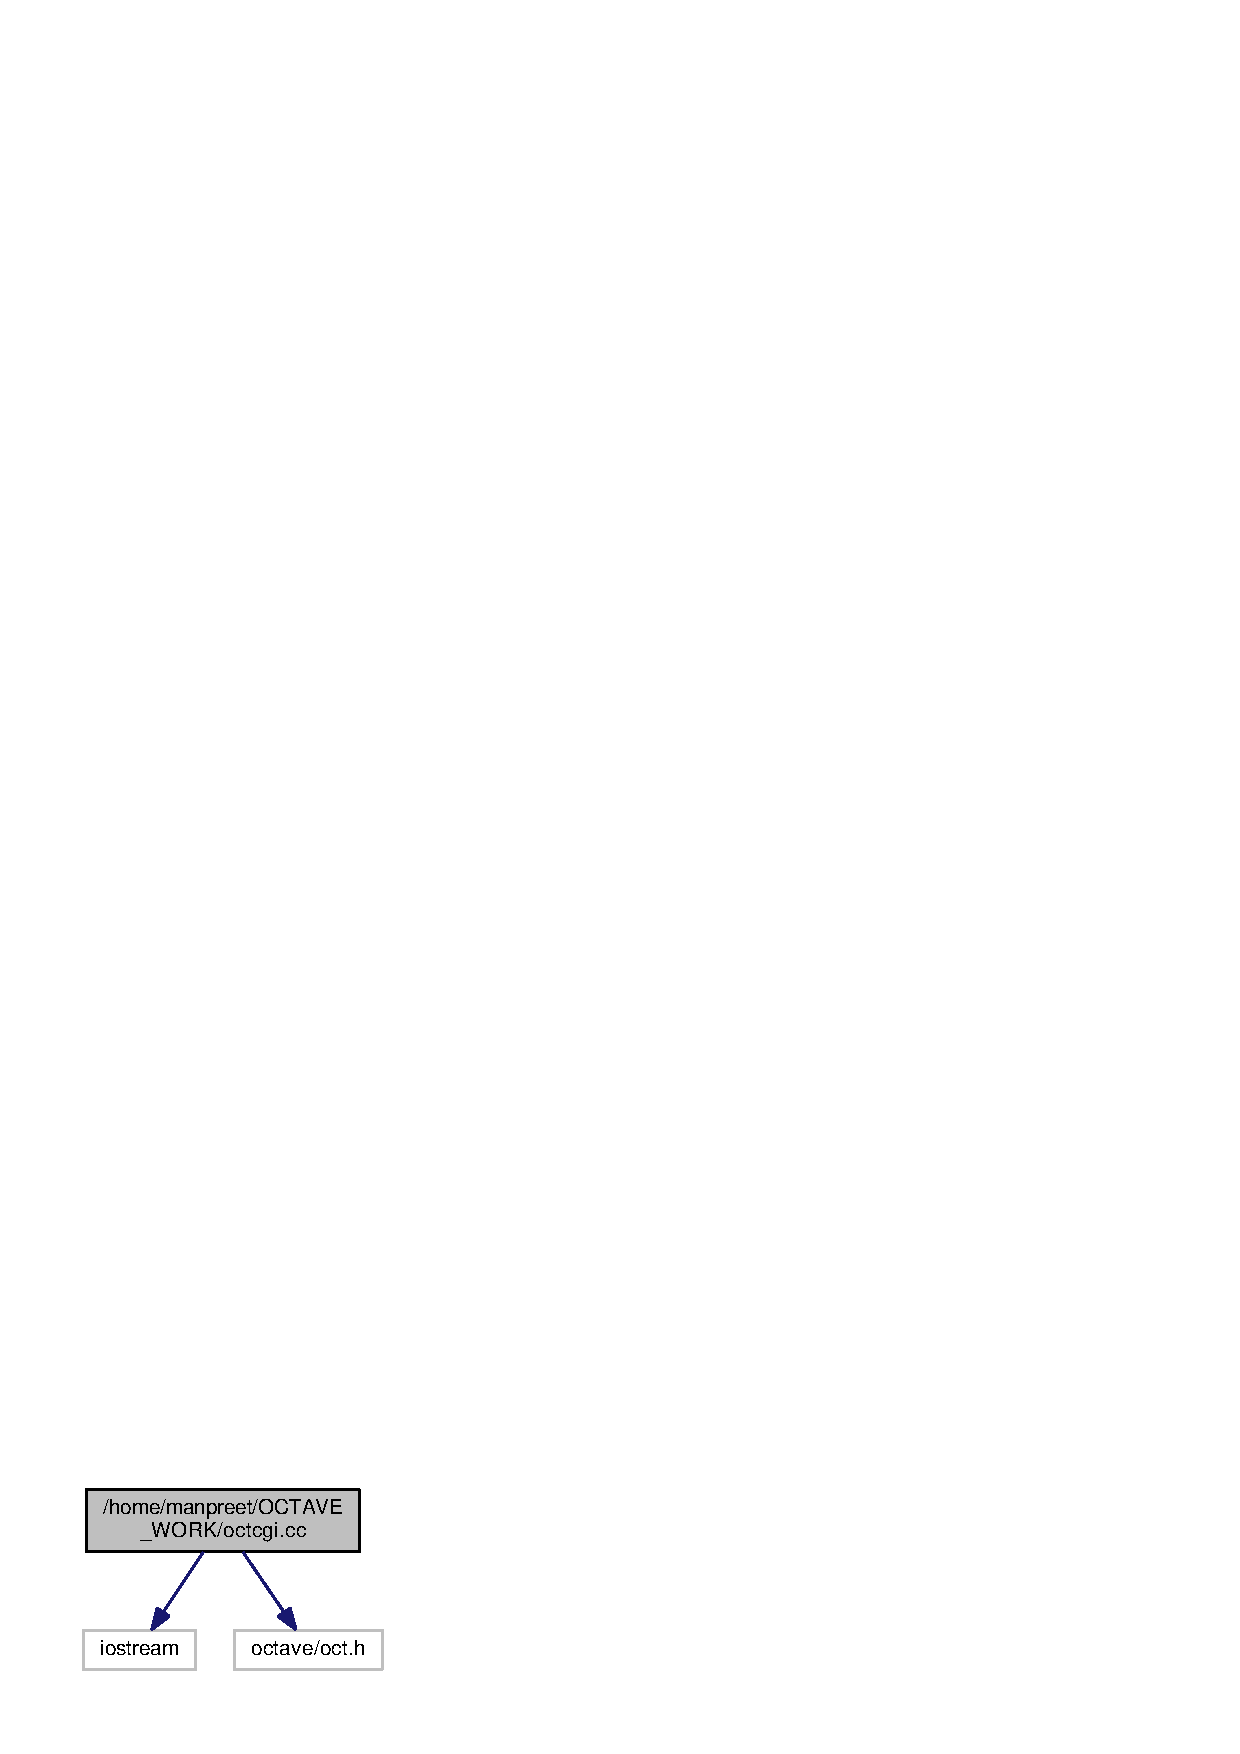
\includegraphics[width=187pt]{octcgi_8cc__incl}
\end{center}
\end{figure}
\subsection*{Functions}
\begin{DoxyCompactItemize}
\item 
int {\bf main} ()
\end{DoxyCompactItemize}


\subsection{Function Documentation}
\index{octcgi.\-cc@{octcgi.\-cc}!main@{main}}
\index{main@{main}!octcgi.cc@{octcgi.\-cc}}
\subsubsection[{main}]{\setlength{\rightskip}{0pt plus 5cm}int main (
\begin{DoxyParamCaption}
{}
\end{DoxyParamCaption}
)}\label{octcgi_8cc_ae66f6b31b5ad750f1fe042a706a4e3d4}


Definition at line 4 of file octcgi.\-cc.



References i.


\begin{DoxyCode}
5 \{
6   std::cout << \textcolor{stringliteral}{"Hello Octave world!\(\backslash\)n"};
7 
8   \textcolor{keywordtype}{int} n = 2;
9   Matrix a\_matrix = Matrix (n, n);
10 
11   \textcolor{keywordflow}{for} (octave\_idx\_type i = 0; i < n; i++)
12     \textcolor{keywordflow}{for} (octave\_idx\_type j = 0; j < n; j++)
13       a\_matrix(i,j) = (i + 1) * 10 + (j + 1);
14 
15   std::cout << a\_matrix;
16 
17   \textcolor{keywordflow}{return} 0;
18 \}
\end{DoxyCode}

\section{/home/manpreet/\-O\-C\-T\-A\-V\-E\-\_\-\-W\-O\-R\-K/result.cc File Reference}
\label{result_8cc}\index{/home/manpreet/\-O\-C\-T\-A\-V\-E\-\_\-\-W\-O\-R\-K/result.\-cc@{/home/manpreet/\-O\-C\-T\-A\-V\-E\-\_\-\-W\-O\-R\-K/result.\-cc}}
{\ttfamily \#include $<$iostream$>$}\\*
Include dependency graph for result.\-cc\-:\nopagebreak
\begin{figure}[H]
\begin{center}
\leavevmode
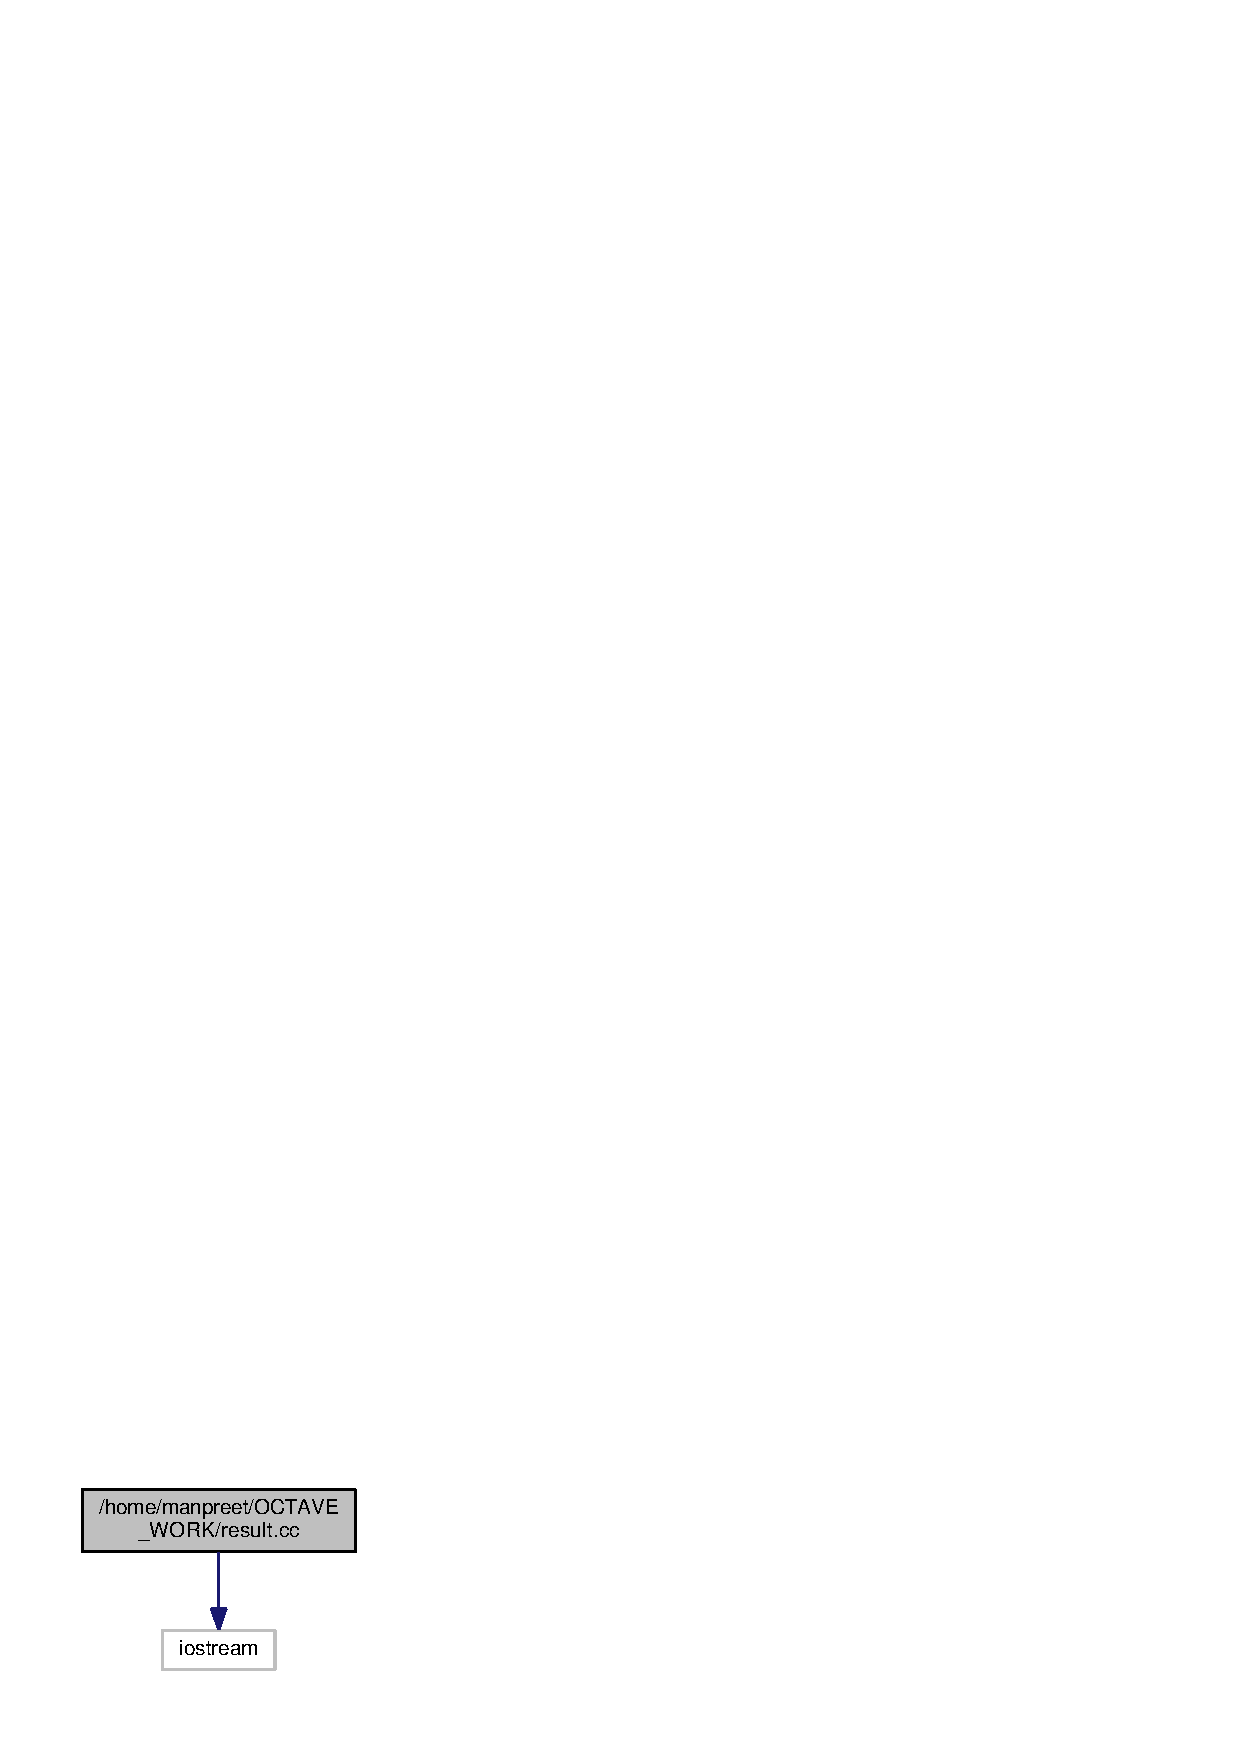
\includegraphics[width=174pt]{result_8cc__incl}
\end{center}
\end{figure}
\subsection*{Functions}
\begin{DoxyCompactItemize}
\item 
int {\bf main} ()
\end{DoxyCompactItemize}


\subsection{Function Documentation}
\index{result.\-cc@{result.\-cc}!main@{main}}
\index{main@{main}!result.cc@{result.\-cc}}
\subsubsection[{main}]{\setlength{\rightskip}{0pt plus 5cm}int main (
\begin{DoxyParamCaption}
{}
\end{DoxyParamCaption}
)}\label{result_8cc_ae66f6b31b5ad750f1fe042a706a4e3d4}


Definition at line 3 of file result.\-cc.


\begin{DoxyCode}
4 \{
5 \textcolor{keywordtype}{int} accno,choice,c,damt,wamt,bal, cur\_bal;
6 cout<<\textcolor{stringliteral}{"enter your account number and current balance\(\backslash\)n"};
7 cin>>accno>>bal;
8 cout<<\textcolor{stringliteral}{"press 1 for deposit\(\backslash\)n"};
9 cout<<\textcolor{stringliteral}{"press 2 for withdraw"};
10 cin>>c;
11 \textcolor{keywordflow}{switch}(c)
12 \{
13 \textcolor{keywordflow}{case} 1:
14  cout<<\textcolor{stringliteral}{"enter amount  that you want to deposit\(\backslash\)n"};
15  cin>>damt;
16  cur\_bal=bal+damt;
17 cout<<\textcolor{stringliteral}{" your current balance after deposit is="}<< cur\_bal;
18  \textcolor{keywordflow}{break};
19 
20 \textcolor{keywordflow}{case} 2:
21  cout<<\textcolor{stringliteral}{"enter amount that you want to withdraw\(\backslash\)n"};
22  cin>>wamt;
23  cur\_bal=bal-wamt;
24  cout<<\textcolor{stringliteral}{" Balance after deduction is ="}<< wamt<<\textcolor{stringliteral}{"\(\backslash\)n"};
25  \textcolor{keywordflow}{break};
26 cout<<\textcolor{stringliteral}{"\(\backslash\)n"};
27 \}
28 \}
\end{DoxyCode}

\section{/home/manpreet/\-O\-C\-T\-A\-V\-E\-\_\-\-W\-O\-R\-K/transpose.m File Reference}
\label{transpose_8m}\index{/home/manpreet/\-O\-C\-T\-A\-V\-E\-\_\-\-W\-O\-R\-K/transpose.\-m@{/home/manpreet/\-O\-C\-T\-A\-V\-E\-\_\-\-W\-O\-R\-K/transpose.\-m}}
\subsection*{Functions}
\begin{DoxyCompactItemize}
\item 
{\bf dlmwrite} (\char`\"{}matrix.\-txt\char`\"{}, M)
\end{DoxyCompactItemize}
\subsection*{Variables}
\begin{DoxyCompactItemize}
\item 
{\bf M} =rand(4,4)
\end{DoxyCompactItemize}


\subsection{Function Documentation}
\index{transpose.\-m@{transpose.\-m}!dlmwrite@{dlmwrite}}
\index{dlmwrite@{dlmwrite}!transpose.m@{transpose.\-m}}
\subsubsection[{dlmwrite}]{\setlength{\rightskip}{0pt plus 5cm}dlmwrite (
\begin{DoxyParamCaption}
\item[{\char`\"{}matrix.\-txt\char`\"{}}]{, }
\item[{{\bf M}}]{}
\end{DoxyParamCaption}
)}\label{transpose_8m_abceec1db81c0f73b595b18dff5b45352}


\subsection{Variable Documentation}
\index{transpose.\-m@{transpose.\-m}!M@{M}}
\index{M@{M}!transpose.m@{transpose.\-m}}
\subsubsection[{M}]{\setlength{\rightskip}{0pt plus 5cm}M =rand(4,4)}\label{transpose_8m_aad05f78187c942f9dd521605fa81f1ba}


Definition at line 1 of file transpose.\-m.


%--- End generated contents ---

% Index
\newpage
\phantomsection
\addcontentsline{toc}{chapter}{Index}
\printindex

\end{document}
